\chapter[Achieving Max-min Fairness in Distributed Job Execution with Task Transmissions]{Achieving Max-min Fairness in Distributed Job Execution with Task Transmissions}
\label{ch:DAMF}

In this chapter, we study the problem of achieving max-min fair resource allocation in distributed job execution with task transmissions. The problem includes both computing the resource allocation and assigning the demand transmission across the system, so that the aggregate resource allocation is fair among jobs. We focus on the online setting where jobs arrive dynamically for execution. Our goal is to achieve better fairness of resource allocation among jobs, while improving the system utilization.

%We first present a system model and then define the problem of Dynamic Aggregate Max-min Fairness (DAMF). We prove that DAMF is achievable and satisfies the properties of Pareto efficiency, envy-freeness and strategy-proofness. We then propose an algorithm to achieve DAMF and analyze its time complexity. Finally, we discuss how to apply DAMF to online scenarios where jobs arrive dynamically.

%%%%%%%%%%%%%%%%%
\section{System Model}
\label{sec:model_1}
Consider a geo-distributed system composed of $m$ separate sites: $S_1, S_2, ..., S_m$. Each site $S_j$ holds compute resources with a capacity $u_j$. The capacity can be interpreted as the volume of computing slots that are available.

We would like to conduct fair resource allocations among jobs in an online environment where jobs arrive dynamically for execution. To do so, we start by studying a static problem of defining and deriving a fair instantaneous resource allocation among active jobs at a certain snapshot of the system. Suppose $n$ jobs $J_1, J_2, ..., J_n$ are running in the system. Each job $J_i$ consists of tasks that process distinct data partitions and could run in parallel. Due to the data locality consideration, initially each task is restricted to be served at a certain site where the input data is available. Therefore, a job's resource demand on a site $S_j$ can be defined as the total demand of its tasks that can only run on $S_j$. For instance, if each task needs one computing slot for execution, the resource demand on site $S_j$ is given by the number of tasks to run on $S_j$. We model the resource demands of all jobs as an $n*m$ demand matrix $D_{n*m}$, where each element $d_{ij}$ denotes job $J_i$'s demand on site $S_j$. Similarly, the instantaneous resource allocations to all jobs on all sites can be represented by an $n*m$ allocation matrix $A_{n*m}$, where each element $a_{ij}$ denotes how much resource job $J_i$ is allocated on site $S_j$. Throughout this dissertation, we shall use capital letters to stand for matrices and corresponding small letters to stand for the elements therein. For simplicity, we use $[x]$ to represent the set $\{1, 2, \dots, x\}$ for a positive integer $x$. 

Some basic constraints should be met to ensure that $A_{n*m}$ is a sensible allocation. First, the summation of allocated resources on any site should not exceed that site's capacity:
\begin{equation}
    \forall j\in [m], \quad \sum_{i=1}^n a_{ij} \leq u_j.
\label{eq:allocfeas}
\end{equation}
Allocations satisfying (\ref{eq:allocfeas}) are said {\em feasible}. 

Second, any job's allocation on any site should not exceed its demand on that site so that no resources are wasted:
\begin{equation}
    \forall i\in[n], j\in[m], \quad 0\leq a_{ij}\leq d_{ij}.
\label{eq:allocrati}
\end{equation}
Allocations satisfying (\ref{eq:allocrati}) are said {\em rational}. 

Suppose there are networks connecting the sites so that they can be used to transfer data and hence demand for compute resources from one site to another. We use an $n*m$ transmission matrix $\Delta D_{n*m}$ to represent the demand transmissions. Each element $\Delta d_{ij}$ can be positive or negative: A positive $\Delta d_{ij}$ describes how much demand of job $J_i$ is transferred into site $S_j$, while a negative $\Delta d_{ij}$ means some demand is transferred out of (removed from) site $S_j$, and $\Delta d_{ij} = 0$ represents no transmission. Apparently, we cannot transfer more demand out of a site than what a given job has at that site:
\begin{equation}
    \forall i\in[n], j\in[m], \quad d_{ij} + \Delta d_{ij} \geq 0,
\label{eq:trx1}
\end{equation}
and the overall demand of each job $J_i$ should be kept unchanged after the transmissions:
\begin{equation}
    \forall i\in[n], \quad \sum_{j=1}^m \Delta d_{ij}=0.
\label{eq:trx2}
\end{equation}
We assume that the primary bandwidth bottleneck of the system lies in the link through which each site connects to the backbone network. Thus, to model the available network capacity, we use a count limit $c_j$ for each site $S_j$ to describe an upper bound on the total demand that can be transferred into and out of site $S_j$ within a predefined short period of time $T$: (note that the data partition required by tasks of different jobs can be different, we add a weight $w_i$ to each job denoting the relative data partition ratio between tasks of different jobs):
\begin{equation}
    \forall j\in[m], \quad \sum_{i=1}^n |w_i \Delta d_{ij}| \leq c_j. %
\label{eq:trx3}
\end{equation}
More specifically, suppose the average data partition size is $0.5$ GB, the system time threshold $T=10$ and the link bandwidth is $0.2$ GB/s, then the count limit $c_j$ at a site $S_j$ is $0.2*10/0.5 = 4$. Furthermore, suppose three jobs $J_1$, $J_2$ and $J_3$ has data partition size $0.25$ GB, $0.5$ GB and $1$ GB, respectively; Then, the data partition weight for each job is $w_1 = 0.25/0.5 = 0.5$, $w_2 = 0.5/0.5=1$, $w_3 = 1/0.5=2$, and the constraint is $0.5 d_{1j} + d_{2j} + 2 d_{3j} < 4$.

In big data processing frameworks, each task typically processes a data partition/split of the same size \cite{copart}. The transmission count limit $c_j$ can be computed based on the data partition size, the amount of bandwidth currently available, and $T$. 

Upon the transmissions, each job $J_i$'s demand on site $S_j$ becomes $d_{ij} + \Delta d_{ij}$, i.e., the demand matrix becomes $D + \Delta D$. Hence, constraint (\ref{eq:allocrati}) is rewritten as:
\begin{equation}
    \forall i\in[n], j\in[m], \quad 0\leq a_{ij}\leq d_{ij}+\Delta d_{ij}.
\label{eq:new_rational}
\end{equation}

We shall start with defining and deriving a fair resource allocation $A_{n*m}$ among jobs satisfying constraints (\ref{eq:allocfeas}), (\ref{eq:trx1}), (\ref{eq:trx2}), (\ref{eq:trx3}) and (\ref{eq:new_rational}), given the demands $D_{n*m}$, site capacities $u_j$'s and transfer limits $c_j$'s. Later, we shall discuss how to apply the solution to this static problem to online scenarios where jobs arrive dynamically. The key notations used in this paper are summarized in Table \ref{tab:Notation_1}. 

\begin{table}[htb]
\centering 
\caption{Notation Table}
\label{tab:Notation_1}
\begin{tabular}{l l} 
 \hline
 Notation & Definition \\
 \hline
 $\mathcal M = \{S_1, S_2, ..., S_m\}$ & Set of sites \\ 
 $\mathcal J = \{J_1, J_2, ..., J_n\}$ & Set of jobs\\ 
 $w_i$ & Job $J_i$'s data partition weight \\
 $u_j$ & Site $S_j$'s compute resource capacity\\
 $c_j$ & Site $S_j$'s transmission count limit\\
 $D_{n*m}$ & Demand matrix\\
 $\Delta D_{n*m}$ & Transmission matrix \\
 $A_{n*m}$ & Allocation matrix \\
 $\mathcal X$ & Set of all allocation matrices \\
 $X$ & Set of all aggregate allocation vectors \\
 \hline
\end{tabular}
\end{table}

\begin{figure}[htbp]
  \centering
  \begin{subfigure}[t]{0.32\textwidth}
    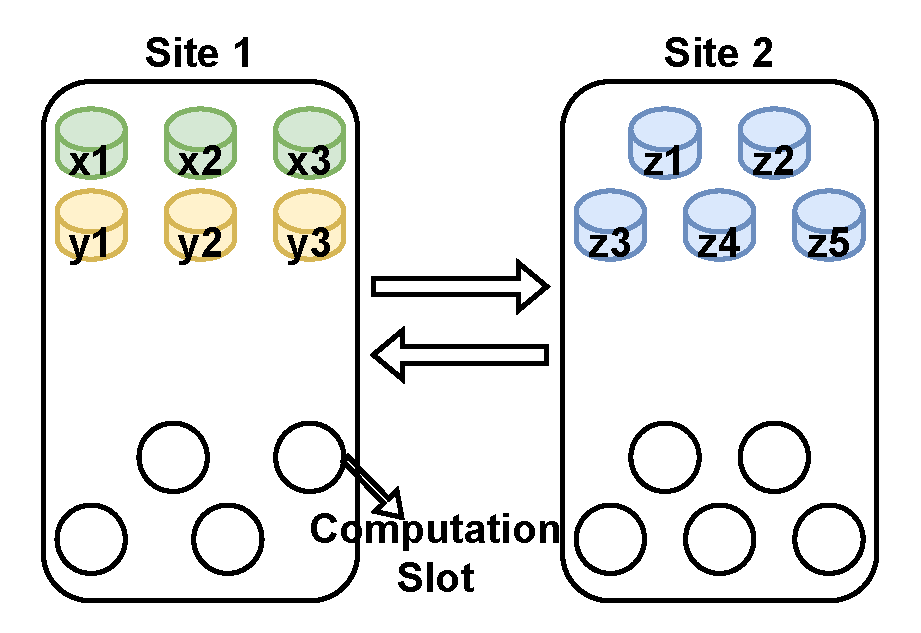
\includegraphics[width=\textwidth]{Image/Eg1.drawio.pdf}
    \caption{Initial system state}
    \label{Fg:eg1}
  \end{subfigure}
  \hfill
  \begin{subfigure}[t]{0.32\textwidth}
    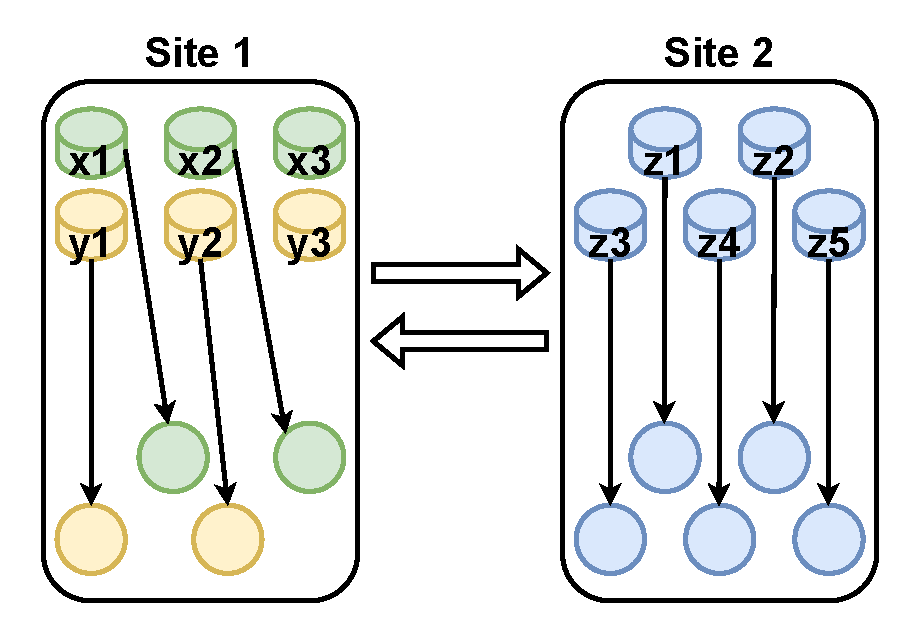
\includegraphics[width=\textwidth]{Image/Eg2.drawio.pdf}
    \caption{Fair allocation without transmission}
    \label{Fg:eg2}
  \end{subfigure}
  \hfill
  \begin{subfigure}[t]{0.32\textwidth}
    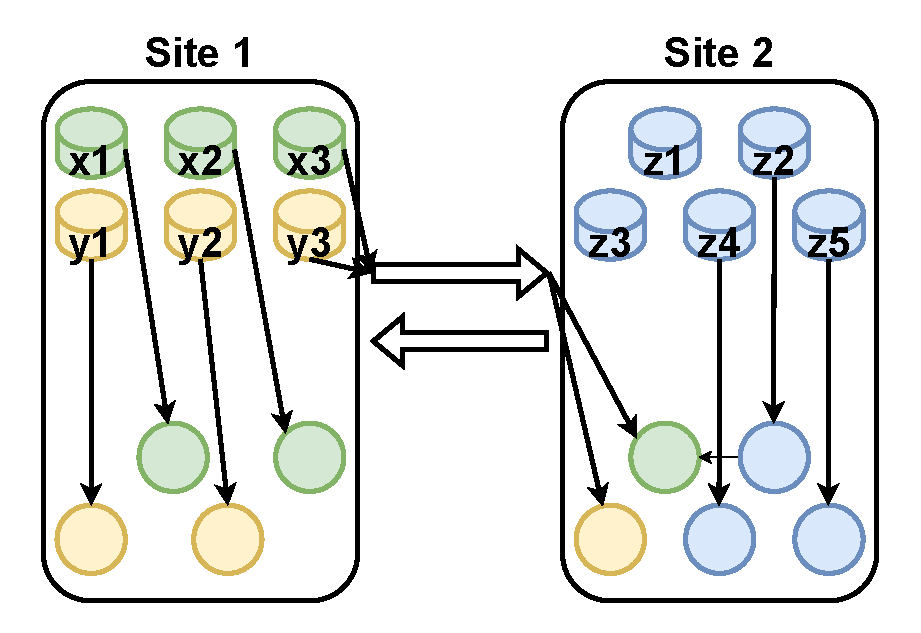
\includegraphics[width=\textwidth]{Image/Eg3.drawio.pdf}
    \caption{Fair allocation utilizing network resources}
    \label{Fg:eg3}
  \end{subfigure}
  \caption{An intuitive example}
  \label{fig:Motivation_eg}
\end{figure}

Figure \ref{fig:Motivation_eg} provides an example of the static problem to illustrate that transferring job demands can help improve the fairness of resource allocation. Suppose a geo-distributed system has 2 sites $S_1$ and $S_2$ with capacities of $4$ and $5$ computing slots respectively. There are three active jobs $x$, $y$ and $z$ in the system. As shown in Figure \ref{Fg:eg1}, jobs $x$ and $y$ have $3$ tasks each, where the input data is available on site $S_1$; job $z$ has $5$ tasks, where the input data is available on site $S_2$. If no demand can be transferred between sites, the most balanced resource allocation among jobs $x$, $y$ and $z$ is $2$, $2$ and $5$ computing slots as illustrated in Figure \ref{Fg:eg2}, because jobs $x$ and $y$ do not have demands on site $S_2$. With a transfer limit of $2$, we can transfer one task of job $x$ and one task of job $y$ from $S_1$ to $S_2$, and allocate them with computing slots on $S_2$. As a result, all jobs $x$, $y$ and $z$ are allocated $3$ computing slots each as shown in Figure \ref{Fg:eg3}, which is more balanced (fair) from the global perspective.


\section{Preliminaries}
\label{sec3:prelim}
\subsection{Max-min Fairness}
Max-Min Fairness (MMF) is one of the most common resource allocation strategies, which takes ``serving the most unsatisfied user'' as priority. Considering the resource allocation among $n$ jobs as an $n$-dimensional vector, MMF can be defined as follows \cite{radunovic2007unified}:

\begin{definition}
    \label{def:MMF}
    Consider a set $V$ of n-dimensional vectors. A vector $\vec x \in V$ is max-min fair on set $V$, if and only if for any $\vec y \in V$, if $y_s > x_s$ for an index $s \in \{1, 2, ..., n\}$, there must exist another index $t \in \{1, 2, ..., n\}$ such that $y_t < x_t \leq x_s$.
\end{definition}

Based on the above definition, if we want to increase a component $x_s$ in a max-min fair vector $\vec x$ while keeping the new vector staying in the vector set $V$, we must decrease another component $x_t$ in $\vec x$ whose original value is less than or equal to that of $x_s$. The max-min fair vector is unique if it exists, because if there are multiple max-min fair vectors within a given vector set $V$, we can derive contradiction simply by applying the definition of MMF to them. Clearly, the max-min fair vector does not exist in every vector set. Previous work has proved sufficient conditions for the existence of the max-min fair vector \cite{radunovic2007unified}. 
\begin{theorem}
    If a set $V$ is compact and convex, then it is max-min achievable.
\label{the:achievable}
\end{theorem}

\subsection{Aggregate Max-min Fairness}
A naive idea of applying MMF to distributed job execution is to consider each site independently and find the MMF resource allocation among jobs on each site based on their local demands. This policy is known as Independent Max-min Fairness (IMF) \cite{AMF}. However, IMF can be far away from providing fair services to jobs from the global perspective due to the possibly unbalanced distribution of job demands and compute capacities among sites.

Guan \textit{et al.} \cite{AMF} defined Aggregate Max-min Fairness (AMF) for distributed job execution and presented an algorithm to achieve AMF. AMF treats the distributed system as a united resource pool and constructs an aggregate allocation vector to represent each job's total resource allocation across all distributed sites: 
$$\vec{A} = \langle \sum_{j=1}^m a_{1j},  \sum_{j=1}^m a_{2j}, ..., \sum_{j=1}^m a_{nj} \rangle.$$
AMF requires this vector to be max-min fair among all possible aggregation vectors. While the AMF vector is unique if it exists, there may be multiple ways of resource allocation by sites to jobs producing this AMF vector since the vector only specifies each job's aggregate allocation across all sites. 

AMF does not consider utilizing network resources to transfer job demands between sites. Transferring job demands has the potential to improve the fairness of compute resource allocation for jobs as well as the system utility.

\section{Dynamic Aggregate Max-min Fairness}
\label{sec:DAMF}
We propose a new resource allocation policy called Dynamic Aggregate Max-min Fairness (DAMF) to improve the fairness of resource allocation by making use of network resources. Given the demand matrix, site capacities and transfer limits, there are a variety of possible transmission matrices and each would give rise to a number of feasible and rational allocations. Under this circumstance, DAMF requires the aggregate allocation vector to be max-min fair among all the vectors derived from the allocation matrices resulting from all possible transmission matrices. Let $\mathcal{X}$ be the set of all feasible and rational allocation matrices under all possible transmission matrices, and $X$ be the set of all aggregate allocation vectors drawn from $\mathcal{X}$. DAMF can be formally defined as follows:

\begin{definition}
    An allocation $A_{n*m}$ satisfies Dynamic Aggregate Max-min Fairness, if and only if its aggregate allocation vector $\vec A$ is max-min fair over the set $X$.
\end{definition}

We prove that DAMF exists by showing the compactness and convexity of set $X$. 
\begin{lemma}
    The set $X$ is compact.
\label{lem:compact}
\end{lemma}

\begin{proof}
Consider any aggregate allocation vector $\vec{A} = \langle\sum_{j=1}^m a_{1j}, \allowbreak $ $\sum_{j=1}^m a_{2j},\allowbreak \dots, \allowbreak \sum_{j=1}^m a_{nj}\rangle$ derived from some allocation matrix $A$ under some demand matrix $D + \Delta D$ after transmission. According to constraints (\ref{eq:allocfeas}), (\ref{eq:new_rational}) and (\ref{eq:trx2}), for the \textit{i}-th component $\sum_{j=1}^m a_{ij}$, we have $0 \leq \sum_{j=1}^m a_{ij} \leq \sum_{j=1}^m \min\{u_j, d_{ij} +\Delta d_{ij}\} \leq \sum_{j=1}^m \min\{u_j, d_{ij} +c_j\}$. Thus, the set $X$ is closed and bounded. Hence, it is compact.
\end{proof}

\begin{lemma}
    The set $X$ is convex.
\label{lem:convex}
\end{lemma}

\begin{proof}
Based on the definition of convexity, we need to prove that for any two vectors $\vec A, \vec B \in X$ and any $0 \leq \lambda \leq 1$, it holds that $\lambda \vec A + (1-\lambda) \vec B \in X$.

Let $\mathcal{T}$ be the set of all possible transmission matrices satisfying (\ref{eq:trx1}), (\ref{eq:trx2}) and (\ref{eq:trx3}). We first prove that $\mathcal{T}$ is convex. i.e., for any two transmission matrices $\Delta D,\Delta D' \in \mathcal{T}$ and any $0 \leq \lambda \leq 1$, $\lambda \cdot \Delta D + (1-\lambda) \cdot \Delta D' \in \mathcal{T}$.

Firstly, $\lambda \cdot \Delta D + (1-\lambda) \cdot \Delta D'$ satisfies constraint (\ref{eq:trx1}): since $\Delta D,\Delta D' \in \mathcal{T}$, for each job $J_i$ and each site $S_j$, we have $d_{ij} + \Delta d_{ij} \geq 0$ and $d_{ij} + \Delta d_{ij}' \geq 0$, and hence, 
\begin{align}
    \nonumber &d_{ij} + \lambda \cdot \Delta d_{ij} + (1-\lambda) \cdot \Delta d_{ij}'\\
    \nonumber &= \lambda \cdot (d_{ij} + \Delta d_{ij}) + (1-\lambda) \cdot (d_{ij} + \Delta d_{ij}')\\
    \nonumber &\geq \lambda\cdot 0+(1-\lambda)\cdot 0 =0. 
\end{align}

Similarly, it can be shown that $\lambda \cdot \Delta D + (1-\lambda) \cdot \Delta D'$ satisfies constraints (\ref{eq:trx2}) and (\ref{eq:trx3}). As a result, $\lambda \cdot \Delta D + (1-\lambda) \cdot \Delta D' \in \mathcal{T}$ and thus, $\mathcal{T}$ is a convex set.

Next, suppose the original demand matrix is $D$, and vector $\vec A$ and $\vec B$'s corresponding allocation and transmission matrices are $\{A, \Delta D^A\}$ and $\{B, \Delta D^B\}$, respectively. Since the set $\mathcal{T}$ is convex, we have $\lambda \cdot \Delta D^A + (1-\lambda) \cdot \Delta D^B \in \mathcal{T}$. By definition, $\lambda \vec A + (1-\lambda) \vec B$ is the aggregate allocation vector for the allocation matrix $\lambda A + (1-\lambda) B$. We prove that $\lambda A + (1-\lambda) B$ is a rational and feasible allocation matrix for the demand matrix $D + \lambda \cdot \Delta D^A + (1-\lambda) \cdot \Delta D^B$.

Since $A$ and $B$ are feasible, by constraint (\ref{eq:allocfeas}) we have
\begin{align}
    \forall j \in [m], \quad \nonumber\sum_{i=1}^n a_{ij} \leq u_j, \quad \nonumber\sum_{i=1}^n b_{ij} \leq u_j.
\end{align}
Thus,
\begin{align}
    \nonumber \sum_{i=1}^n\left(\lambda a_{ij} + (1-\lambda)b_{ij}\right) &\leq \lambda u_j+ (1-\lambda) u_j =u_j.
\end{align}
Hence, $\lambda A + (1-\lambda)B$ is feasible. Similarly, it can be shown that $\lambda A + (1-\lambda)B$ is rational. Therefore, $\lambda A + (1-\lambda)B \in \mathcal{X}$. As a result, $\lambda \vec A + (1-\lambda) \vec B \in X$, and $X$ is a convex set.
\end{proof}
Lemmas \ref{lem:compact} and \ref{lem:convex} together with Theorem \ref{the:achievable} give rise to the following conclusion:
\begin{theorem}
    Dynamic Aggregate Max-min Fairness is achievable.
\label{the:DAMFachievable}
\end{theorem}

\section{Properties of DAMF}
\label{sec:property}
In this section, we study whether DAMF satisfies the properties of Pareto efficiency, envy-freeness and strategy-proofness, which are well-accepted characteristics of fairness. %\sout{ and sharing incentive}.
\subsection{Pareto Efficiency}
Pareto efficiency means that no further improvement can be achieved which makes at least one individual better off without making any other individual worse off \cite{DRF}. This includes two aspects \cite{gutman2012GDF}: first, no resource required by any consumer is left idle; second, no consumer is allocated any resource that it does not need.

In our distributed job execution context, suppose the DAMF vector and its corresponding allocation matrix are $\vec A$ and $A_{n*m}$ respectively. Pareto efficiency means that for any other feasible and rational allocation matrix $A'_{n*m}$ and its corresponding aggregate allocation vector $\vec A'$, if there is an index $i$ such that the $i$-th component of $\vec A$ is larger than the $i$-th component of $\vec A'$, i.e., $\sum_{j=1}^m a'_{ij} > \sum_{j=1}^m a_{ij}$, there must be another index $k$ such that the $k$-th component of $\vec A$ is smaller than the $k$-th component of $\vec A'$, i.e., $\sum_{j=1}^m a'_{kj} < \sum_{j=1}^m a_{kj}$.

\begin{theorem}
    DAMF is Pareto efficient.
\end{theorem}
\begin{proof}
    By definition, the DAMF vector is the max-min fair vector among all possible aggregate allocation vectors under all possible transmission matrices. For any other feasible and rational allocation matrix $A'_{n*m}$ and its corresponding aggregate allocation vector $\vec A'$, if $\sum_{j=1}^m a'_{ij} > \sum_{j=1}^m a_{ij}$ for some job $J_i$, then based on Definition \ref{def:MMF}, there exists another job $J_k$ such that $\sum_{j=1}^m a'_{kj} < \sum_{j=1}^m a_{kj} \leq \sum_{j=1}^m a_{ij}$. Hence, the theorem is proven. 
\end{proof}

\subsection{Envy-freeness}
Envy-freeness means that no individual would envy another individual's allocation. More specifically, in our distributed job execution context, envy-freeness means that for any job $J_l$, its usable allocation will not increase if it is given any other job $J_k$'s transmission and allocation.

\begin{theorem}
    DAMF is envy-free.
\end{theorem}

\begin{proof}
Let $\vec A$ be the DAMF vector, and $A_{n*m}$, $\Delta D_{n*m}$ be its corresponding allocation and transmission matrices respectively.
Assume on the contrary that they are not envy-free, that is, a job $J_l$ will have its usable allocation increased if it is given another job $J_k$'s transmission $\Delta d_{kj}$'s and allocation $a_{kj}$'s. Note that the transmission refers to the network bandwidth allocated, and $J_l$ does not have to fully utilize the allocated bandwidth in order to optimize its usable allocation. Let $r_{lj}$'s be the actual transmission used by $J_l$, where for each site $S_j$, $|r_{lj}| \leq |\Delta d_{kj}|$ (transmission is within the allocated bandwidth), $d_{lj} + r_{lj} \geq 0$ (transmission is feasible), and $\sum_{j=1}^m r_{lj} = 0$ (the overall demand of $J_l$ is unchanged after transmission). Then, the demands of $J_l$ on all sites would become $d_{lj} + r_{lj}$'s. Thus, $J_l$'s usable allocation on each site $S_j$ is $\min\{d_{lj}+r_{lj}, a_{kj}\}$. If $J_l$'s total usable allocation over all sites increases, it means that
$$
\sum_{j=1}^m \min\{d_{lj}+r_{lj}, a_{kj}\} > \sum_{j=1}^m a_{lj}.
$$
This implies two facts:

(i) By eliminating the $\min$ operator, we have
$$
\sum_{j=1}^m a_{kj} > \sum_{j=1}^m a_{lj},
$$
which means job $J_k$'s aggregate allocation is larger than $J_l$'s aggregate allocation in the DAMF vector.

(ii) There must be at least one site $S_{j'}$ such that $\min\{d_{lj'}+r_{lj'}, a_{kj'}\} > a_{lj'}$, which indicates $d_{lj'}+r_{lj'} > a_{lj'}$ and $a_{kj'} > a_{lj'}$. The former inequality means that $J_l$'s demand on site $S_{j'}$ is not completely satisfied, and the latter inequality means that $J_k$'s allocation on site $S_{j'}$ is larger than $J_l$'s allocation on $S_{j'}$. 

By (ii), from the DAMF allocation matrix $A_{n*m}$, we could increase $a_{lj'}$ by decreasing $a_{kj'}$ on site $S_{j'}$. Accordingly, $J_l$'s aggregate allocation increases while $J_k$'s aggregate allocation decreases. Note that by (i), $J_k$'s aggregate allocation is larger than $J_l$'s aggregate allocation in $A_{n*m}$. This implies that we can increase the $l$-th component of the DAMF vector $\vec A$ by decreasing its $k$-th component which is larger, and this contradicts the fact that $\vec A$ is the max-min fair vector among all possible aggregate allocation vectors.
\end{proof}

\subsection{Strategy-proofness}
Strategy-proofness means that no individual could achieve better allocation by lying about its demand. In our distributed job execution context, strategy-proofness requires that no job could get higher usable allocation by lying about its demand $d_{ij}$'s, even if this would cause the recomputation of the transmission matrix $\Delta D$ and the allocation matrix $A$.

\begin{theorem}
    DAMF is strategy-proof.
\end{theorem}

\begin{proof}
Let $\vec A$ be the DAMF vector, and $A_{n*m}$, $\Delta D_{n*m}$ be its corresponding allocation and transmission matrices derived from the true demand matrix $D_{n*m}$ (i.e., when all jobs are honest). Let $D'_{n*m}$ be the misclaimed demand matrix when a job $J_l$ lies about its demand, and $A'_{n*m}$ and $\Delta D'_{n*m}$ be the resultant allocation matrix and transmission matrix respectively. Note that the transmission refers to the network bandwidth allocated. $J_l$ does not have to fully utilize the allocated bandwidth in order to optimize its usable allocation. Let $r_{lj}$'s be the actual transmission used by $J_l$, where for each site $S_j$, $|r_{lj}| \leq |\Delta d'_{lj}|$ (transmission is within the allocated bandwidth), $d_{lj} + r_{lj} \geq 0$ (transmission is feasible for $J_l$'s true demand), and $\sum_{j=1}^m r_{lj} = 0$ (the overall demand of $J_l$ is unchanged after transmission). For notational convenience, we define $R$ as the transmission matrix actually used by all jobs, i.e., $R$ replaces $\Delta d'_{lj}$'s with $r_{lj}$'s for job $J_l$ and keeps all other elements unchanged in $\Delta D'$. Then, the real demand matrix after transmission is given by $D + R$. In particular, the real demands of $J_l$ at all sites are $d_{lj} + r_{lj}$'s. Thus, $J_l$'s usable allocation on each site $S_j$ is $\min\{d_{lj}+r_{lj}, a'_{lj}\}$. We prove that $J_l$'s total usable allocation over all sites cannot increase, i.e.,
$$
\sum_{j=1}^m \min\{d_{lj}+r_{lj}, a'_{lj}\} \leq \sum_{j=1}^m a_{lj}. 
$$

We prove it by contradiction. Assume on the contrary that $J_l$'s total usable allocation over all sites increases: 
\begin{equation}
\sum_{j=1}^m \min\{d_{lj}+r_{lj}, a'_{lj}\} > \sum_{j=1}^m a_{lj}.
\label{eq:strategy1}
\end{equation}
It follows that 
\begin{equation}
\sum_{j=1}^m a'_{lj} >\sum_{j=1}^m a_{lj}.
\label{eq:strategy4}
\end{equation}

Since $J_l$ lies, it is possible that it gets excessive allocation than its real demand on some sites. Next, we construct a rational allocation matrix $B'$ by shrinking $J_l$'s excessive allocation (if any) in $A'$ to its real demand:

(i) For each job $J_i \neq J_l$, let $b'_{ij} = a'_{ij}$. Since these jobs are honest about their demands, their allocations must be rational: 
$$\forall j \in [m], \quad b'_{ij} = a'_{ij} \leq d_{ij}+\Delta d'_{ij} = d_{ij}+ r_{ij}.$$

(ii) For job $J_l$, if its allocation $a'_{lj}$ on site $S_j$ does not exceed its real demand $d_{lj} + r_{lj}$, it is kept the same in $B'$:
$$\forall j \in[m] \text{~where~} a'_{lj} \leq d_{lj} + r_{lj}, \quad b'_{lj} = a'_{lj}.$$
    
(iii) For job $J_l$, if its allocation $a'_{lj}$ on site $S_j$ exceeds its real demand $d_{lj} + r_{lj}$, we shrink it to be the real demand in $B'$:
$$\forall j \in [m] \text{~where~} a'_{lj} > d_{lj} + r_{lj}, \quad b'_{lj} = d_{lj} + r_{lj}.$$

In short, $B'$ records the allocations in $A'$ that can be actually used by all jobs. It is clear that $B'$ is a feasible and rational allocation matrix given the real demand matrix $D + R$.
For simplicity, $B'$ can be uniformly written as follows:
$$
\forall i \in [n], j \in [m], \; b'_{ij} = \min\{d_{ij}+r_{ij}, a'_{ij}\}.
$$

It then follows from (\ref{eq:strategy1}) that
\begin{equation}
\sum_{j=1}^m b'_{lj} >\sum_{j=1}^m a_{lj},
\label{eq:strategy2}
\end{equation}
which means that $J_l$'s aggregate allocation increases from $A$ to $B'$.

By definition, $A$'s aggregate allocation vector $\vec A$ is the max-min fair vector over all possible allocation matrices including those under the real demand matrix $D + R$. Based on the definition of max-min fairness and (\ref{eq:strategy2}), there must be another job $J_{i_1}$ whose aggregate allocation in $A$ is no larger than $J_l$ and whose aggregate allocation decreases from $A$ to $B'$:
$$
\sum_{j=1}^m a_{lj} \geq \sum_{j=1}^m a_{i_1j} > \sum_{j=1}^m b'_{i_1j}.
$$

Clearly, $J_{i_1}$ is different from $J_l$. Thus, by the above construction, $J_{i_1}$'s allocations in $B'$ and $A'$ are the same. Hence, the inequality above can be rewritten as:
\begin{equation}
\sum_{j=1}^m a_{lj} \geq \sum_{j=1}^m a_{i_1j} > \sum_{j=1}^m a'_{i_1j}.
\label{eq:strategy3}
\end{equation}

Next, we construct another allocation matrix $B$ based on $A$ assuming that the demand matrix is $D'+R$ (which is the demand matrix used to derive $A'$): 

(i) For each job $J_i \neq J_l$, let $b_{ij} = a_{ij}$.

(ii) For job $J_l$, if its allocation $a_{ij}$ on site $S_j$ does not exceed the demand $d'_{lj}+r_{lj}$, it is kept the same in $B$: $b_{lj} = a_{lj}$.

(iii) For job $J_l$, if its allocation $a_{ij}$ on site $S_j$ exceeds the demand $d'_{lj} +r_{lj}$, we shrink it to be the latter demand in $B$: $b_{lj} = d'_{ij} +r_{ij}$.

In short, $B$ is built by shrinking $J_l$'s allocation in $A$ exceeding the demand in $D'+R$ to the latter:
$$
\forall i \in [n], j \in [m], \; b_{ij} = \min\{d'_{ij}+r_{ij}, a_{ij}\}.
$$

Since $J_{i_1}$ is different from $J_l$,  $J_{i_1}$'s allocations in $B$ and $A$ are the same: $\sum_{j=1}^m a_{i_1j} =\sum_{j=1}^m b_{i_1j}$. Together with (\ref{eq:strategy3}), it can be inferred that $J_{i_1}$'s aggregate allocation increases from $A'$ to $B$, \textit{i.e.}, 
\begin{equation}
\sum_{j=1}^m b_{i_1j} > \sum_{j=1}^m a'_{i_1j}.
\label{eq:strategy8}
\end{equation}

Note that both $A'$ and $B$ are based on the demand matrix $D' + R$ and are feasible and rational. By definition, the aggregate allocation vector of $A'$ is the max-min fair vector over all possible allocation matrices including those under the demand matrix $D' + R$. Since $J_{i_1}$'s aggregate allocation increases from $A'$ to $B$, based on the definition of max-min fairness, there must be another job $J_{i_2}$ whose aggregate allocation in $A'$ is no larger than $J_{i_1}$ and whose aggregate allocation decreases from $A'$ to $B$:
\begin{equation}
\sum_{j=1}^m a'_{i_1 j} \geq \sum_{j=1}^m a'_{i_2 j} > \sum_{j=1}^m b_{i_2 j}.
\label{eq:strategy5}
\end{equation}

Clearly, $J_{i_2}$ is different from $J_{i_1}$. In addition, by (\ref{eq:strategy4}), (\ref{eq:strategy3}) and (\ref{eq:strategy5}), we have
\begin{equation}
\sum_{j=1}^m a'_{l j} > \sum_{j=1}^m a'_{i_1 j} \geq \sum_{j=1}^m a'_{i_2 j}.
\label{eq:strategy0}
\end{equation}
Thus, $J_{i_2}$ is also different from $J_l$. Hence, $J_l$, $J_{i_1}$ and $J_{i_2}$ are three distinct jobs.

By the construction of $B$, $J_{i_2}$'s allocations in $B$ and $A$ are the same. Moreover, by the construction of $B'$, $J_{i_2}$'s allocations in $B'$ and $A'$ are also the same. Therefore, (\ref{eq:strategy5}) implies that:
\begin{equation}
\sum_{j=1}^m b'_{i_2 j} > \sum_{j=1}^m a_{i_2 j},
\label{eq:strategy6}
\end{equation}
which means that $J_{i_2}$'s aggregate allocation increases from $A$ to $B'$. 

Now we can repeat the above analysis. Similar to the argument following (\ref{eq:strategy2}), based on the definition of max-min fairness for $A$ and (\ref{eq:strategy6}), there must be another job $J_{i_3}$ whose aggregate allocation in $A$ is no larger than $J_{i_2}$ and whose aggregate allocation decreases from $A$ to $B'$:
$$
\sum_{j=1}^m a_{i_2j} \geq \sum_{j=1}^m a_{i_3j} > \sum_{j=1}^m b'_{i_3j}.
$$

Similarly, it can be shown that $J_{i_3}$ is different from any of the jobs $J_l$, $J_{i_1}$ and $J_{i_2}$. Since $J_{i_3}$ is different from $J_l$, its allocations keep the same from $A$ to $B$ and from $A'$ to $B'$. Therefore, $J_{i_3}$'s aggregate allocation increases from $A'$ to $B$:
\begin{equation}
\sum_{j=1}^m b_{i_3j} > \sum_{j=1}^m a'_{i_3j}.
\label{eq:strategy7}
\end{equation}

Then, similar to the argument following (\ref{eq:strategy8}), 
based on the definition of max-min fairness for $A'$ and (\ref{eq:strategy7}), there must be another job $J_{i_4}$ whose aggregate allocation in $A'$ is no larger than $J_{i_3}$ and whose aggregate allocation decreases from $A'$ to $B$:
$$
\sum_{j=1}^m a'_{i_3j} \geq \sum_{j=1}^m a'_{i_4j} > \sum_{j=1}^m b_{i_4j}.
$$

Similar to (\ref{eq:strategy0}), it can be shown that $J_{i_4}$ is different from any of the jobs $J_l$, $J_{i_1}$, $J_{i_2}$, $J_{i_3}$, and 
\begin{equation}
\sum_{j=1}^m a'_{l j} > \sum_{j=1}^m a'_{i_1 j} \geq \sum_{j=1}^m a'_{i_2 j} > \sum_{j=1}^m a'_{i_3 j} \geq \sum_{j=1}^m a'_{i_4 j}.
\label{eq:strategy9}
\end{equation}
Since $J_{i_4}$ is different from $J_l$, its allocations keep the same from $A$ to $B$ and from $A'$ to $B'$. Therefore, $J_{i_4}$'s aggregate allocation increases from $A$ to $B'$:
$$
\sum_{j=1}^m b'_{i_4j} > \sum_{j=1}^m a_{i_4j}.
$$

By repeating the above process continuously, we can obtain an infinite sequence of jobs $J_{i_1}, J_{i_2}, J_{i_3}, J_{i_4}, J_{i_5}, J_{i_6}, \dots$ with non-increasing aggregate allocations in $A'$ like (\ref{eq:strategy9}), which contradicts that there are a finite number of jobs. Hence, the theorem is proven.
\end{proof}

% 请确保在 LaTeX 文件的导言区（Preamble）引入了该宏包：
% \usepackage[linesnumbered,ruled,vlined]{algorithm2e}

\begin{algorithm}[htbp]
\caption{Computing DAMF Allocation}\label{alg:basic}

    % 1. 输入输出与初始化 (不再使用 \STATE)
    \KwIn{A set of sites $\{S_1, S_2, ..., S_m\}$ with capacities $\{u_1, u_2, \dots, u_m\}$ and transfer limits $\{c_1, c_2, \dots, c_m\}$; a set of jobs $\{J_1, J_2, \dots, J_n\}$ with data partition weights $\{w_1, w_2, \dots, w_n\}$ and demand matrix $D$}
    \KwOut{A DAMF allocation matrix $A$; a transmission matrix $\Delta D$}
    
    \BlankLine % 插入一个空行隔开初始化
    $A \leftarrow \textbf{0}$\;
    $\Delta D \leftarrow \textbf{0}$\;
    $\mathcal{J} \leftarrow \{J_1, J_2, ..., J_n\}$\;
    \BlankLine

    % 2. 主循环结构 (花括号包裹，删除了 \ENDWHILE)
    \While{$\mathcal{J} \neq \emptyset$}{
        Solve the following linear program:\;
        \quad Maximize $T$, subject to:\;
        \quad\quad $\forall J_i \in \mathcal{J} : \sum^m_{j=1}a_{ij} \geq T$\;
        \quad\quad $\forall J_i \notin \mathcal{J} : \sum^m_{j=1}a_{ij} = t_i$\;
        \quad\quad $\forall j \in [m]: \sum^n_{i=1}a_{ij} \leq u_j$\;
        \quad\quad $\forall i \in [n], j \in [m]: 0 \leq a_{ij} \leq d_{ij}+\Delta d_{ij}$\;
        \quad\quad $\forall j \in [m]: \sum_{i=1}^n |w_i\Delta d_{ij}| \leq c_j$\;
        \quad\quad $\forall i \in [n]: \space \sum_{j=1}^m \Delta d_{ij}=0$\;
        
        Let $T_{max}$ be the outcome of the above linear program\;
        \BlankLine
        
        % For 循环 (删除了 \ENDFOR)
        \For{each $J_l \in \mathcal{J}$}{
            % If - Else If 结构 (\Eclif) 
            \eIf{$\sum^m_{j=1} d_{lj} = T_{max}$}{
                $t_l \leftarrow T_{max}$\;
                $\mathcal{J} \leftarrow \mathcal{J} \setminus\{J_l\}$\;
            }{
                \If{$\sum^m_{j=1} a_{lj}= T_{max} \text{ and } (\forall j \in [m], a_{lj} = d_{lj} \lor \sum^n_{i=1}a_{ij}=u_j)$}{
                    Check the feasibility of the following program:\;
                    \quad $\sum_{j=1}^n a_{lj} > T_{max}$\;
                    \quad $\forall J_i \in \mathcal{J} \land i \neq l: \sum^m_{j=1}a_{ij}=T_{max}$\;
                    \quad $\forall J_i \notin \mathcal{J} : \sum^m_{j=1}a_{ij}=t_i$\;
                    \quad $\forall j \in [m]: \sum^n_{i=1}a_{ij} \leq u_j$\;
                    \quad $\forall i \in [n], j \in [m]: 0 \leq a_{ij} \leq d_{ij}+\Delta d_{ij}$\;
                    \quad $\forall j \in [m]: \sum_{i=1}^n |w_i\Delta d_{ij}| \leq c_j$\;
                    \quad $\forall i \in [n]: \space \sum_{j=1}^m \Delta d_{ij}=0$\;
                    \BlankLine
                    
                    \If{the above program is infeasible}{
                        $t_l \leftarrow T_{max}$\;
                        $\mathcal{J} \leftarrow \mathcal{J} \setminus\{J_l\}$\;
                    }
                }
            }
        }
    }
    \BlankLine
    \Return $A_{n \times m}, \Delta D_{n \times m}$\;
\end{algorithm}

% \section{Achieving DAMF}
% \label{sec:algo}
% \subsection{Algorithm for Computing DAMF Allocation}

% \begin{algorithm}[htbp]
% \caption{Computing DAMF Allocation}\label{alg:basic}
% \begin{algorithmic}[1]

% \STATE \textbf{Input}: A set of sites $\{S_1, S_2, ..., S_m\}$ with capacities and transfer limits $\{c_1, c_2, \dots, c_j\}$; a set of jobs $\{J_1, J_2, ..., J_n\}$ with demand matrix $D$; 
% \STATE \textbf{Output}: A DAMF allocation matrix $A$; a transmission matrix $\Delta D$;
% \STATE \textbf{Initialization}: $A \leftarrow \textbf{0}$; $\Delta D \leftarrow \textbf{0}$; $\mathcal{J} \leftarrow \{J_1, J_2, ..., J_n\}$;

% \WHILE{$\mathcal{J} \neq \emptyset$}
%     \STATE Solve the following linear program:
%     \STATE \quad Maximize $T$, subject to: 
%     \STATE \quad $\forall J_i \in \mathcal{J} : \sum^m_{j=1}a_{ij} \geq T$;
%     \STATE \quad $\forall J_i \notin \mathcal{J} : \sum^m_{j=1}a_{ij} = t_i$;
%     \STATE \quad $\forall j \in [m]: \sum^n_{i=1}a_{ij} \leq u_j$;
%     \STATE \quad $\forall i \in [n], j \in [m]: 0 \leq a_{ij} \leq d_{ij}+\Delta d_{ij}$;
%     \STATE \quad $\forall j \in [m]: \sum_{i=1}^n |\Delta d_{ij}| \leq c_j$;
%     \STATE \quad $\forall i \in [n]: \space \sum_{j=1}^m \Delta d_{ij}=0$;
%     \STATE Let $T_{max}$ be the outcome of the above linear program;
    
%     \FOR{each $J_l \in \mathcal{J} $}
%         \IF{$\sum^m_{j=1} d_{lj} = T_{max}$}
%             \STATE $t_l \leftarrow T_{max}$;
%             \STATE $\mathcal{J} \leftarrow \mathcal{J} \setminus\{J_l\}$; 
%         \ELSIF{$\sum^m_{j=1} a_{lj}= T_{max} \text{ and } (\forall j \in [m], a_{lj} = d_{lj} \lor \sum^n_{i=1}a_{ij}=u_j)$}
%             \STATE Check the feasibility of the following program:
%             \STATE \quad $\sum_{j=1}^n a_{lj} > T_{max}$;
%             \STATE \quad $\forall J_i \in \mathcal{J} \land i \neq l: \sum^m_{j=1}a_{ij}=T_{max}$;
%             \STATE \quad $\forall J_i \notin \mathcal{J} : \sum^m_{j=1}a_{ij}=t_i$;
%             \STATE \quad $\forall j \in [m]: \sum^n_{i=1}a_{ij} \leq u_j$;
%             \STATE \quad $\forall i \in [n], j \in [m]: 0 \leq a_{ij} \leq d_{ij}+\Delta d_{ij}$;
%             \STATE \quad $\forall j \in [m]: \sum_{i=1}^n |\Delta d_{ij}| \leq c_j$;
%             \STATE \quad $\forall i \in [n]: \space \sum_{j=1}^m \Delta d_{ij}=0$;
            
%             \IF{the above program is infeasible}
%                 \STATE $t_l \leftarrow T_{max}$;
%                 \STATE $\mathcal{J} \leftarrow \mathcal{J} \setminus\{J_l\}$;
%             \ENDIF
%         \ENDIF
%     \ENDFOR
% \ENDWHILE

% \STATE \textbf{return} $A_{n \times m}, \Delta D_{n \times m}$;
% \end{algorithmic}
% \end{algorithm}

We now design an iterative algorithm (Algorithm \ref{alg:basic}) to compute the DAMF allocation, inspired by the max-min programming method from \cite{radunovic2007unified} which can find the max-min fair allocation vector for any max-min achievable set. The basic idea is to simultaneously increase the allocations of all jobs. Once a job's demand is completely satisfied, the algorithm fixes its allocation and continues to increase the allocations of other jobs. The algorithm terminates when all job demands are satisfied or all available resources are used up.

Each iteration of our algorithm consists of two stages. In stage 1, we define a unified lower bound $T$ and maximize it by increasing the aggregate allocations of all jobs in set $\mathcal{J}$ simultaneously, where $\mathcal{J}$ is the set of jobs whose aggregate allocations have not been fixed yet. Initially, $\mathcal{J}$ contains all jobs (line 3). The maximum $T$ value is derived by solving a linear program which models the constraints of resource allocation introduced in Section \ref{sec:model_1} (lines 5-12), where $t_i$ is the aggregate allocation of a job $J_i$ that has been fixed. 

Let $T_{max}$ denote the maximum $T$ value obtained in stage~1. In stage 2, we identify jobs whose aggregate allocations are to be fixed. If a job $J_l$'s total demand is equal to $T_{max}$ amount of resources, it is fully satisfied. Thus, the algorithm fixes its aggregate allocation to be $T_{max}$ and removes it from $\mathcal{J}$ (lines 15-17). Otherwise, the algorithm checks whether it is possible to increase $J_l$'s aggregate allocation beyond $T_{max}$ without violating other jobs' allocations. If $J_l$'s aggregate allocation from stage 1 is already larger than $T_{max}$, or there exists a site on which $J_l$'s demand is not fully satisfied and the site has spare capacity (i.e., the condition in line 18 is not satisfied), clearly $J_l$'s aggregate allocation can be further increased. Otherwise, we change the aggregate allocation constraints for $J_l$ and other jobs by replacing "$\geq$" with "$>$" (line 20) and "$=$" (line 21) respectively, and then check whether the new linear program has any feasible solution (lines 19-26). If so, it implies that $J_l$'s allocation can be increased and $J_l$ will be kept in set $\mathcal{J}$. Otherwise, $J_l$'s aggregate allocation is fixed at $T_{max}$ and $J_l$ is removed from set $\mathcal{J}$ (lines 27-29). Note that this $T_{max}$ value is the aggregate resource amount, which means that $J_l$'s allocations on individual sites could vary in subsequent iterations as long as the aggregate amount is kept. The algorithm terminates when $\mathcal{J}$ becomes empty (line 4).

The linear program in Algorithm \ref{alg:basic} has $2mn$ variables and $2m+2n+mn$ constraints, where $m$ and $n$ are the numbers of sites and jobs respectively. Since there can be up to $n$ iterations and each iteration needs to solve up to $n$ linear programs in stage 2, the worst-case time complexity of Algorithm \ref{alg:basic} is $O(n^2*LP(2mn,2m+2n+mn))$, where $LP(2mn,2m+2n+mn)$ is the complexity for solving a linear program with $2mn$ variables and $2m+2n+mn$ constraints. 

\subsection{A Fast Approximation}
Algorithm 1 computes an exact DAMF allocation. However, its complexity could raise concern since solving large-scale linear programs can
be computationally expensive \cite{complexity_lip}. In this section, we propose a heuristic algorithm to derive a near-DAMF allocation with significantly reduced time complexity to enhance the practicality.

% 请确保在 LaTeX 文件的导言区（Preamble）引入了该宏包：
% \usepackage[linesnumbered,ruled,vlined]{algorithm2e}

\begin{algorithm}[htbp]
\caption{Heuristic to Approximate DAMF Allocation}\label{alg:approx}

    % 1. 输入输出与初始化
    \KwIn{A set of sites $\{S_1, S_2, ..., S_m\}$ with capacities $\{u_1, u_2, \dots, u_m\}$ and transfer limits $\{c_1, c_2, \dots, c_m\}$; a set of jobs $\{J_1, J_2, \dots, J_n\}$ with data partition weights $\{w_1, w_2, \dots, w_n\}$ and demand matrix $D$;}
    \KwOut{An allocation matrix $A$; a transmission matrix $\Delta D$;}
    
    \BlankLine
    $A = \textbf{0}$\;
    $\Delta D = \textbf{0}$\;
    $\vec{p} = \textbf{0}$\;
    Sort all sites in increasing order of the number of jobs with demands on each site (i.e., the cardinality of $\{J_i: a_{ij} > 0\}$)\; 
    \BlankLine

    % 2. 第一层嵌套 For 循环
    \For{each site $S_j$ in the sorted order}{
        Compute max-min fair allocation $\langle a_{1j}, a_{2j}, ..., a_{nj}\rangle$ on $S_j$ based on job demands $\{d_{1j}, d_{2j}, ..., d_{nj}\}$, capacity $u_j$ of $S_j$, and current aggregate allocation vector $\vec{p} = \langle p_{1}, p_{2}, ..., p_{n}\rangle$ as described in the main text\;
        
        \For{$i \in [n]$}{
            $p_i = p_i + a_{ij}$\;
        }
    }
    \BlankLine
    
    % 3. 集合赋值
    $\mathcal{S}_{spare} = \{ S_j~|~ \sum_{i=1}^n a_{ij} < u_j\}$\;
    $\mathcal{S}_{full} = \{ S_j~|~ \sum_{i=1}^n d_{ij} > u_j\}$\;
    $\mathcal{J} = \{ J_i~|~ \sum_{j=1}^m d_{ij} > \sum_{j=1}^m a_{ij}\}$\;
    \BlankLine

    % 4. 双层嵌套 While 循环
    \While{$\mathcal{S}_{spare} \neq \emptyset \land \mathcal{S}_{full} \neq \emptyset \land \mathcal{J} \neq \emptyset$}{
        Remove all $S_l$'s from $\mathcal{S}_{spare}$ and $\mathcal{S}_{full}$ that $c_l \le \min_{1\le i \le n}{w_i}$ or $\sum_{i=1}^n (d_{il} + \Delta d_{il}) = u_l$\;
        
        \While{$\mathcal{J} \neq \emptyset$}{
            Select job $J_x \in \mathcal{J}$ with the least aggregate allocation\;
            
            \eIf{$\forall S_j \in \mathcal{S}_{full}, d_{xj} + \Delta d_{xj} \leq a_{xj}$}{
                Remove $J_x$ from $\mathcal{J}$\;
            }{
                Select a site $S_y \in \mathcal{S}_{full}$ where $d_{xy} + \Delta d_{xy}> a_{xy}$\; 
                Select a site $S_z \in \mathcal{S}_{spare}$\;
                $\Delta d_{xy} = \Delta d_{xy} - 1$\;
                $\Delta d_{xz} = \Delta d_{xz} + 1$\;
                $a_{xz} = a_{xz} + 1$\;
                $c_y = c_y - w_x$\;
                $c_z = c_z - w_x$\;
                \break
            }
        }
    }
    \BlankLine
    \Return $A_{n*m}, \Delta D_{n*m}$\;
\end{algorithm}

% \begin{algorithm}[htbp]
% \caption{Heuristic to Approximate DAMF Allocation}\label{alg:approx}
% \begin{algorithmic}[1]

% \STATE \textbf{Input}: A set of sites $\{S_1, S_2, ..., S_m\}$ with capacities and transfer limits; a set of jobs $\{J_1, J_2, ..., J_n\}$ with demand matrix $D$;
% \STATE \textbf{Output}: An allocation matrix $A$; a transmission matrix $\Delta D$;
% \STATE \textbf{Initialization}: $A = \textbf{0}$; $\Delta D = \textbf{0}$; $\vec{p} = \textbf{0}$; sort all sites in increasing order of the number of jobs with demands on each site (i.e., the cardinality of $\{J_i: a_{ij} > 0\}$); 
% \FOR{each site $S_j$ in the sorted order}
% \STATE Compute max-min fair allocation $\langle a_{1j}, a_{2j}, ..., a_{nj}\rangle$
% on $S_j$ based on job demands $\{d_{1j}, d_{2j}, ..., d_{nj}\}$, capacity $u_j$ of $S_j$, and current aggregate allocation vector $\vec{p} = \langle p_{1}, p_{2}, ..., p_{n}\rangle$ as described in the main text;
% \FOR {$i \in [n]$}
% \STATE $p_i = p_i + a_{ij}$;
% \ENDFOR
% \ENDFOR
% \STATE $\mathcal{S}_{spare} = \{ S_j~|~ \sum_{i=1}^n a_{ij} < u_j\}$;
% \STATE $\mathcal{S}_{full} = \{ S_j~|~ \sum_{i=1}^n d_{ij} > u_j\}$;
% \STATE $\mathcal{J} = \{ J_i~|~ \sum_{j=1}^m d_{ij} > \sum_{j=1}^m a_{ij}\}$;
% \WHILE{$\mathcal{S}_{spare} \neq \emptyset \land \mathcal{S}_{full} \neq \emptyset \land \mathcal{J} \neq \emptyset$}
%     \STATE Remove all $S_l$'s from $\mathcal{S}_{spare}$ and $\mathcal{S}_{full}$ that $c_l = 0$ or $\sum_{i=1}^n (d_{il} + \Delta d_{il}) = u_l$;
% \WHILE{$\mathcal{J} \neq \emptyset$}
% \STATE Select job $J_x \in \mathcal{J}$ with the least aggregate allocation;
% \IF{$\forall S_j \in \mathcal{S}_{full}, d_{xj} + \Delta d_{xj} \leq a_{xj}$}
% \STATE Remove $J_x$ from $\mathcal{J}$;
% \ELSE
% \STATE Select a site $S_y \in \mathcal{S}_{full}$ where $d_{xy} + \Delta d_{xy}> a_{xy}$; 
% \STATE Select a site $S_z \in \mathcal{S}_{spare}$;
% \STATE $\Delta d_{xy} = \Delta d_{xy} - 1$;
% \STATE $\Delta d_{xz} = \Delta d_{xz} + 1$;
% \STATE $a_{xz} = a_{xz} + 1$;
% \STATE $c_y = c_y - 1$;
% \STATE $c_z = c_z - 1$;
% \STATE Break;
% \ENDIF
% \ENDWHILE
% \ENDWHILE
% \STATE \textbf{return} $A_{n*m}, \Delta D_{n*m}$
% \end{algorithmic}
% \end{algorithm}

The heuristic algorithm (Algorithm \ref{alg:approx}) proceeds in two steps. In step 1 (lines 4-9), we find a fast approximation to AMF (i.e., without transferring job demands between sites) in an iterative manner. Each iteration calculates the compute resource allocation for one site $S_j$, given the job demands and compute capacity on this site as well as the aggregate allocation vector $\vec p$ over the sites that have been processed in previous iterations (line 5). Suppose there are $n$ jobs running in the system. Let $\vec p = \langle p_{1}, p_{2}, ..., p_{n}\rangle$ be the current aggregate allocation vector and $\langle d_{1j}, d_{2j}, ..., d_{nj}\rangle$ be the job demands on site $S_j$. We would like to compute an allocation $\langle a_{1j}, a_{2j}, ..., a_{nj}\rangle$ on $S_j$ so that $\langle p_{1}+a_{1j}, p_{2}+a_{2j}, ..., p_{n}+a_{nj}\rangle$ is max-min fair among all possible allocations for the given $\vec p$. If the total demand of all jobs on site $S_j$ is no larger than its capacity, i.e., $\sum_{i=1}^n d_{ij} \leq u_j$, we can simply satisfy the demands of all jobs by setting $a_{ij} = d_{ij}$ for all $i$'s. Otherwise, we sort the jobs in increasing order of $p_{i}$, i.e., $p_{1} \leq p_{2} \leq ... \leq p_{n}$, and the resources on site $S_j$ will be allocated to a prefix of this job sequence by the definition of max-min fairness. If resources are allocated to the first $k$ jobs, the total resources allocated must be no more than 
\begin{equation}
\sum_{i=1}^k \left(\min\{p_{k+1}, p_i+d_{ij}\} - p_i\right),
\label{eq:waterfill}
\end{equation}
because the aggregate resource allocation of each job cannot exceed the given allocation $p_{k+1}$ of the next job ($(k+1)$-th job). Since (\ref{eq:waterfill}) is non-decreasing with $k$, we can use a binary search to find out which jobs will receive resource allocations on $S_j$ to make full use of its capacity $u_j$. After deciding $k$, we solve the equation $\sum_{i=1}^k \left(\min\{C, p_i+d_{ij}\} - p_i\right) = u_j$ to find out the maximum aggregate resource allocation $C$ among these jobs to achieve max-min fairness. Then, the $i$-th job will be allocated $a_{ij} = \min\{C, p_i+d_{ij}\} - p_i$ amount of resources. Apparently, the iterating order of sites has an impact on the final allocation result. Our idea is to sort all sites in increasing order of the number of jobs with demands on the site (line 3). A site demanded by more jobs is considered to have higher potential in balancing the final aggregate allocation, so we process it in a later iteration.

In step 2 (lines 10-30), we utilize the network resources to improve the allocation derived in step 1. It is not difficult to see that there exists a DAMF allocation (represented by a pair of transmission and allocation matrices) such that for every demand unit (one task) transferred, (i) the task involved is allocated compute resources at the destination site; and (ii) the compute resources at the source site are fully allocated. In fact, if a demand unit transferred does not satisfy (i), the transfer can be canceled without affecting the allocation matrix. Similarly, the transfer of a demand unit that violates (ii) can also be canceled and the task can be satisfied by compute resources at the source site. This would increase the compute resource allocation of the job involved without affecting the compute resource allocation of any other job, thereby contradicting that the original allocation is max-min fair.

Based on the observation above, we define two sets $\mathcal{S}_{spare}$ and $\mathcal{S}_{full}$ to record sites with spare capacities and with more job demands than capacities (lines 10-11), and a set $\mathcal{J}$ to record jobs whose demands are not fully satisfied (line 12). Then, we start a loop to transfer job demands from $\mathcal{S}_{full}$ sites to $\mathcal{S}_{spare}$ sites until either $\mathcal{S}_{spare}$, $\mathcal{S}_{full}$ or $\mathcal{J}$ becomes empty (which implies that no further improvement to the allocation can be made). To make effective use of network resources, we would like all job demands transferred to get compute resource allocations at destination sites. Intuitively, a site will not need to participate in transmissions if its bandwidth is used up or its updated local demand equals its capacity. Thus, within the loop, we first remove all such sites from $\mathcal{S}_{spare}$ and $\mathcal{S}_{full}$ (line 14). As a heuristic to approximate max-min fairness, among all jobs whose demands are not completely satisfied, we pick the job $J_x$ with the least aggregate allocation currently (line 16). If $J_x$'s demands are satisfied on all sites in $\mathcal{S}_{full}$ (implying that $J_x$'s unsatisfied demands locates at the sites that have been removed because no more bandwidth is available), we discard $J_x$ and examine the next job with the least aggregate allocation for demand transmission (lines 17-18). Otherwise, we select the source site and destination site for a transfer of $J_x$: the source site can be any site in $\mathcal{S}_{full}$ where $J_x$'s demand is not fully satisfied (line 20), and the destination site can be any site in $\mathcal{S}_{spare}$ (line 21). After deciding a transmission, we update the related matrices and remaining transfer limits (lines 22-26).

The heuristic algorithm does not require solving linear programs and has much lower time complexity. In step 1, it solves $m$ allocation problems separately (where $m$ is the number of sites). In the water-filling-like strategy, sorting takes $O(n \log n)$ time (where $n$ is the number of jobs), and the binary search takes $O(n \log n)$ time as computing (\ref{eq:waterfill}) takes $O(n)$ time. So, the time complexity of each iteration is $O(n \log n)$, and the total time complexity of step 1 is $O(m n \log n)$. In step 2, the algorithm transfers at most $cm/2 = O(m)$ units of job demand (assuming the transfer limits of all sites are a constant $c$). Updating $\mathcal{S}_{spare}$ and $\mathcal{S}_{full}$ takes $O(m)$ time. If we arrange all unsatisfied jobs in $\mathcal{J}$ as a min-heap based on their aggregate allocations, selecting the unsatisfied job with the least aggregate allocation takes $O(1)$ time. Selecting the source and destination sites takes $O(m)$ time. After the demand transfer, updating the min-heap of $\mathcal{J}$ takes $O(\log n)$ time.
Thus, each unit of demand transfer takes $O(m+\log n)$ time. If a source site for the selected job can always be found, the time complexity of step 2 is $O(m(m+\log n))$. If the selected job fails to find a source site for transmission, the job is discarded and updating the min-heap of $\mathcal{J}$ takes $O(\log n)$ time. In the worst case, discarding all such jobs incur a time complexity of $O(n (m + \log n))$. Therefore, the worst-case time complexity of step 2 is $O((m+n) (m+\log n))$. Hence, the overall complexity of the algorithm is $O(m n \log n + m^2)$. In the experiments, we shall empirically evaluate and compare the computation times of Algorithms \ref{alg:basic} and \ref{alg:approx}.

\subsection{Optimizing Job Completion Times}
In addition to providing fair resource allocation from the global perspective, we can further optimize the job completion times. The key idea is that DAMF fixes only the aggregate resource allocation for each job, while the particular allocations at individual sites can still be adjusted. In this case, the completion time of a job can be optimized by assigning the allocation proportionally to its demand at each site. For example, if a job has $2$ and $4$ tasks at two sites respectively and its aggregate allocation by DAMF is $3$ computing slots, then its allocations at the two sites can be set to $1$ and $2$ computing slots, so that the two sites can finish processing their tasks at the same time (to minimize job completion time) if all tasks have the same processing time. Meanwhile, we need to ensure that other jobs can also achieve their DAMF aggregate allocations. The details of our algorithm are shown in Algorithm \ref{alg:qos}.

% 请确保在 LaTeX 文件的导言区（Preamble）引入了该宏包：
% \usepackage[linesnumbered,ruled,vlined]{algorithm2e}

\begin{algorithm}[htbp]
\caption{Optimizing Job Completion Times}\label{alg:qos}

    % 1. 输入输出
    \KwIn{A set of sites $\{S_1, S_2, ..., S_m\}$ with capacities; a set of jobs $\{J_1, J_2, ..., J_n\}$ with demand matrix $D$; the aggregate allocation $e_i$ of each job $J_i$ in a DAMF allocation with corresponding transmission matrix $\Delta D$}
    \KwOut{An optimized allocation matrix $A'$}
    \BlankLine

    % 2. 外层 For 循环
    \For{$k = 1, 2, \dots, n$}{
        Solve the following linear program:\;
        Maximize $y_k$, subject to:\;
        \quad $\forall j \in [m], \sum_{i=1}^n a_{ij} \leq u_j$\;
        \quad $\forall i < k, j \in [m]: a_{ij} = a'_{ij}$\;
        \quad $\forall i \ge k, j \in [m]: 0 \le a_{ij} \le d_{ij}+\Delta d_{ij}$\;
        \quad $\forall i\ge k: \sum_{j=1}^m a_{ij} = e_i$\;
        \quad $\forall j \in [m]: a_{kj} = d_{kj}*y_k+z_{kj}$, $y_k \ge 0$, $z_{kj} \ge 0$\;
        \BlankLine
        
        % 3. 内层 For 循环
        \For{each $j\in[m]$}{
            $a'_{kj} \leftarrow a_{kj}$\;
        }
    }
    \BlankLine
    \Return $A'_{n*m}$\;
\end{algorithm}

% \begin{algorithm}[htbp]
% \caption{Optimizing Job Completion Times}
% \label{alg:qos}
% \begin{algorithmic}[1]

% \STATE \textbf{Input}: A set of sites $\{S_1, S_2, ..., S_m\}$ with capacities; a set of jobs $\{J_1, J_2, ..., J_n\}$ with demand matrix $D$; the aggregate allocation $e_i$ of each job $J_i$ in a DAMF allocation with corresponding transmission matrix $\Delta D$;
% \STATE \textbf{Output}: An optimized allocation matrix $A'$;

% \FOR{$k = 1, 2, \dots, n$}
% \STATE Solve the following linear program:
% \STATE Maximize $y_k$, subject to:
% \STATE \quad $\forall j \in [m], \sum_{i=1}^n a_{ij} \leq u_j$;
% \STATE \quad $\forall i < k, j \in [m]: a_{ij} = a'_{ij}$;
% \STATE \quad $\forall i \ge k, j \in [m]: 0 \le a_{ij} \le d_{ij}+\Delta d_{ij}$;
% \STATE \quad $\forall i\ge k: \sum_{j=1}^m a_{ij} = e_i$;
% \STATE \quad $\forall j \in [m]: a_{kj} = d_{kj}*y_k+z_{kj}$, \;$ y_k \ge 0$, $z_{kj} \ge 0$;
% \FOR{each $j\in[m]$}
% \STATE $a'_{kj} \leftarrow a_{kj}$;
% \ENDFOR
% \ENDFOR
% \STATE \textbf{return} $A'_{n*m}$.
% \end{algorithmic}
% \end{algorithm}

Algorithm \ref{alg:qos} optimizes the completion times of jobs iteratively from $J_1$ to $J_n$. In each iteration, the algorithm solves a linear program (lines 4-10) to optimize the completion time of a job $J_k$. The first constraint of the linear program (line 6) ensures that the allocations are feasible. The second constraint (line 7) retains the allocations of jobs already optimized. The third constraint (line 8) ensures that the allocations of remaining jobs are rational given the input transmission matrix. The fourth constraint (line 9) guarantees that the aggregate allocations of these jobs comply with DAMF. The last constraint (line 10) expresses $J_k$'s allocation $a_{kj}$ at each site $S_j$ as a linear combination $d_{kj}*y_k +z_{kj}$, where $y_k$ is a shared proportional coefficient for all sites and $z_{kj}$ is an auxiliary variable. Thus, by maximizing $y_k$, the resource allocation $a_{kj}$ across sites can be made as close to proportional as possible to the resource demand $d_{kj} + \Delta d_{kj}$ at each site, thereby minimizing job $J_k$'s completion time. After solving the linear program, $J_k$'s allocation at each site is decided and recorded in $A'$ (lines 11-13). Finally, the algorithm returns the optimized allocation $A'$ after all iterations. The set of jobs $\{J_1, J_2, ..., J_n\}$ input to the algorithm can be arranged in different orders based on job arrival times, job priorities, job demands, etc. In this paper, we sort the jobs based on their total demands from low to high so that jobs with smaller numbers of tasks are optimized earlier.

\subsection{Deployment}
\begin{figure}[t]
    \centering
    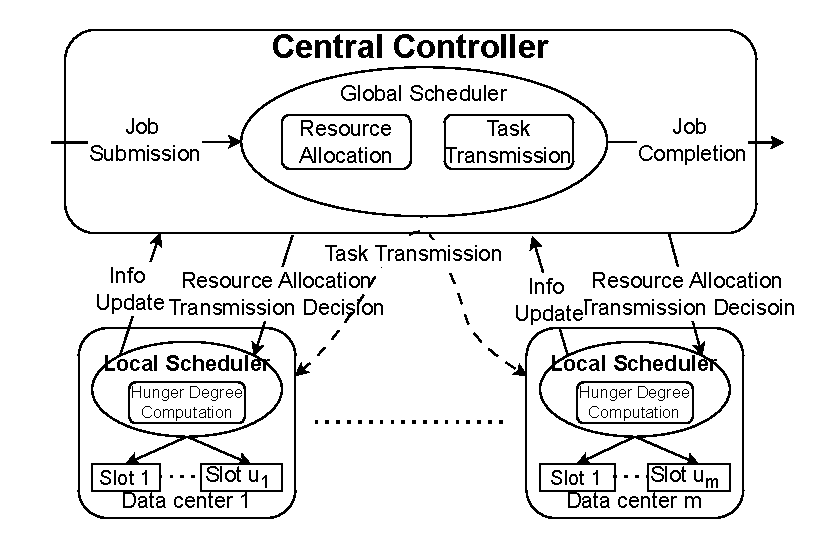
\includegraphics[width=0.7\linewidth]{Image/DAMF.drawio.pdf}
    \caption{System Architecture}
    \label{fig:Architecture}
\end{figure}

Algorithms \ref{alg:basic} and \ref{alg:approx} in the above sections derive a DAMF or near-DAMF resource allocation among active jobs at a snapshot of the system. In this section, we discuss how to apply them to online scenarios where jobs arrive dynamically for execution. As shown in Figure \ref{fig:Architecture}, the algorithm for computing the DAMF allocation can be deployed at a central scheduler of the distributed job execution system. The scheduler tracks the real-time resource capacities of the sites and the distributed demands of each job on all sites. Once an allocation is derived, the scheduler propagates the transmission matrix $\Delta D$ and the allocation matrix $A$ to relevant sites, where job demands (task input data) would be transferred based on $\Delta D$. The compute resource allocation at each site would follow the allocation matrix $A$. If the demand of a job on a site is larger than its allocation on the site, some of its tasks will have to wait. When a computing slot becomes available on a site, the site computes the "Hunger Degree" for jobs with pending tasks locally and selects the job with the lowest Hunger Degree to launch its task in the available slot. More specifically, the Hunger Degree of a job on a site is the ratio between the number of its tasks that are currently running (the number of computing slots occupied by this job now) and its DAMF allocation on this site (the number of computing slots that this job is supposed to occupy). A lower Hunger Degree indicates that the job is taking up less slots than expected and deserves more slot allocation. In particular, if a job's DAMF allocation at a site is zero, its Hunger Degree is set to infinity.



In distributed job execution, the demands of jobs change continuously because of job arrivals and task completions. In general, the completion of a single task would not significantly change the relative distribution of job demands and hence the resultant resource allocation \cite{AMF}. Therefore, to reduce the computational overhead, allocations can be recomputed only when a new job arrives or all tasks of an existing job are completed on some site. Recall that in our model, there is a time threshold $T$ which determines the limit $c_j$ on the total demand that can be transferred into and out of each site $S_j$. This parameter $T$ can be dynamically adjusted according to the job arrival rate. When new jobs arrive frequently, $T$ can be shortened to align with the reduced time between recomputations; conversely, $T$ can be lengthened if the job arrival rate decreases.


\section{Experiments}
\label{sec3:experiment}
Simulation experiments are conducted to compare the fairness and efficiency between various allocation policies. 

\begin{figure}[t]
    \centering
    \subfloat[Alibaba Trace]
    {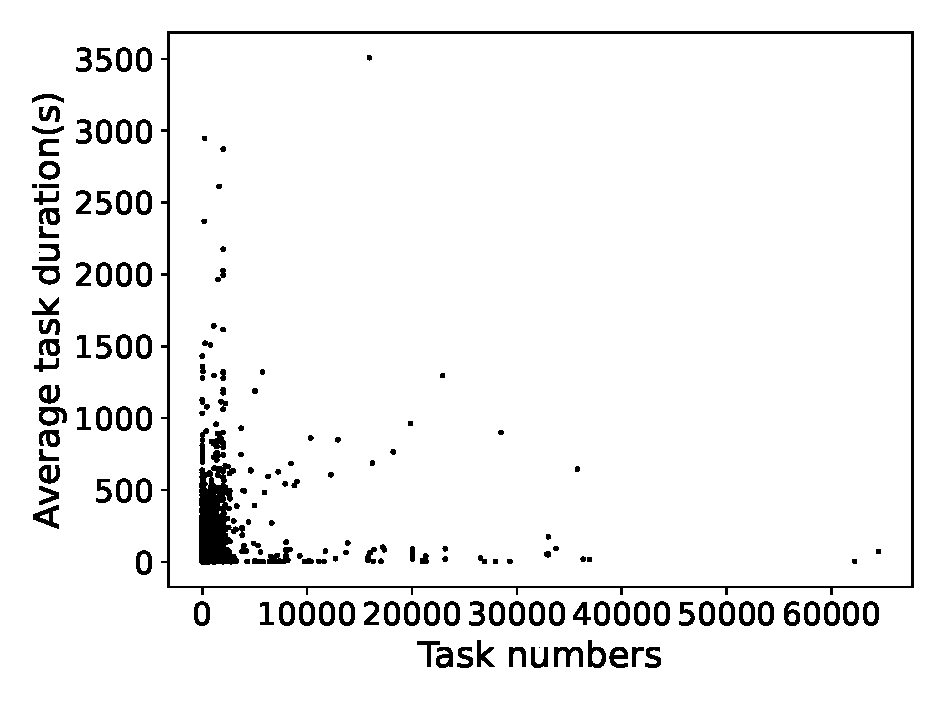
\includegraphics[width=0.48\linewidth]{Image/JobDistribution_Ali2017test2D.eps}%
    }
    \hfil
    \subfloat[Google Trace]
    {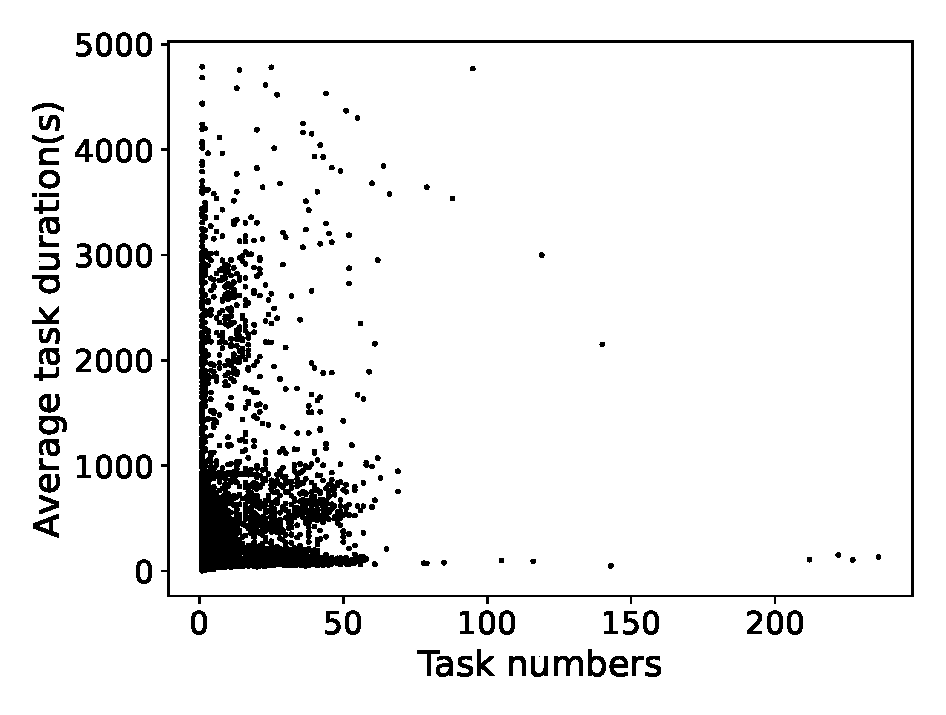
\includegraphics[width=0.48\linewidth]{Image/JobDistribution_Gg2019_112D.eps}%
    }
    \caption{Task characteristics of two datasets}
    \label{fig3:distribution}
\end{figure}

\begin{table}[tb]
\caption{Dataset characteristics}
    \centering
    \begin{tabular}{c c c}
     \toprule
     Dataset & Average task duration & Average task count per job \\
     \midrule
     Alibaba & $155.68$ seconds & $273.5$ tasks \\ 
     
     Google  & $512.25$ seconds & $4.5$ tasks\\ 
     \bottomrule
    \end{tabular}
    \label{tab3:data_characteristics}
\end{table}

\subsection{Datasets}
We use job traces from Alibaba \cite{Ali2017} and Google \cite{Gg2019}. The Alibaba trace contains information on approximately 16 million tasks collected from 1300 machines over a period of 12 hours in August 2017. The Google trace records events (e.g., a task is scheduled, completed or aborted) from Google's eight Borg cells over the month of May 2019. We pre-process the raw traces to extract key information, including the arrival time, task count and task durations of each job. From each trace, a continuous sequence of 15,000 jobs is randomly selected to serve as the dataset driving our simulations.

Figure \ref{fig3:distribution} and Table \ref{tab3:data_characteristics} illustrate the task characteristics of both datasets, including the task number and mean task duration of each job, and the average task duration and task count of all jobs. It can be seen that the jobs in the Alibaba dataset generally have larger numbers of tasks and shorter average task durations, whereas the jobs in the Google dataset tend to have longer average task durations and significantly fewer tasks.

\subsection{System Configuration}
We simulate a distributed system of $m$ sites, each with 32 computing slots. Each task is assumed to take up one computing slot to run and release it after completion. Due to the switching overhead consideration, we assume that there is no preemption during the execution of a task. For each job, the distribution of its tasks among the sites is generated by a Zipf distribution: the numbers of tasks placed on the sites are proportional to $1, \frac{1}{2^\alpha}, \frac{1}{3^\alpha}, ..., \frac{1}{m^\alpha}$, where $\alpha$ is a Zipf parameter. A higher $\alpha$ implies a more skewed distribution (a higher proportion of tasks are concentrated at one site), whereas $\alpha$ = $0.0$ indicates a uniform distribution. In the experiments, we test four Zipf distributions with $\alpha$ set to $0.0$, $0.5$, $1.0$ and $2.0$ to simulate different workload situations. We shuffle the order of the sites when deploying each job's task distribution, so that the overall workload distribution of all jobs is roughly balanced among sites. We scale the job arrival times to simulate different levels of overall system workloads. We experiment with different numbers of sites and different workload levels, and observe similar performance trends. We implement the algorithms and run the experiments on a server with AMD EPYC 7H12 2.6GHz processor and 1024GB memory.

\subsection{Resource Allocation Policies}
\label{resource_policy}
Besides Algorithms \ref{alg:basic} and \ref{alg:approx} (called DAMF and DAMF\_a for short), we also implement three baseline policies: IMF, AMF (both introduced in Section \ref{sec3:prelim}) and Dynamic Independent Max-min Fairness (DIMF). DIMF utilizes network resources on top of IMF: it first applies the IMF policy for resource allocation on each site, then transfers unsatisfied job demands to the sites with spare compute capacities to maximize the system utility (subject to the transfer limits), where jobs with lower aggregate allocations in the first step are assigned higher transmission priority in order to promote fairness. All the policies recompute the allocation matrix only when a new job arrives or an existing job completes all of its tasks on some site. We use CPLEX \cite{Cplex} as the program solver in the experiments. Since a task cannot be transferred fractionally, the transmission matrix $\Delta D$ derived to achieve the DAMF allocation may not be workable. To make DAMF applicable in practice, we enforce the elements of the transmission matrix $\Delta D$ in Algorithm \ref{alg:basic} to be integers, i.e., replacing the linear program with a mixed-integer program. This would incur extra but acceptable computation time. We shall demonstrate the computation times of DAMF and DAMF\_a later. Note that DAMF\_a does not need to apply a similar modification because the transmission matrix $\Delta D$ derived from its heuristic is always integral.

As introduced in Section \ref{sec:model_1}, transmission count limit $c$ is computed based on the average data partition size $S$, available bandwidth $B$ and time threshold $T$: $c = BT/S$. In the experiments, we set $T$ = 50 seconds (which is small compared to the average task duration shown in Table \ref{tab3:data_characteristics}), $S$ = 1GB and $B$ = 160Mbps or 480Mbps for all sites, thus $c = (160\; \text{or}\;480)*50/(1*1024*8) \approx 1\; \text{or}\; 3$. Under these settings, a task transmission generally takes $50/ (1\;\text{or}\;3)=50\;\text{or}\;16.67$ seconds to arrive at its destination. To emulate the bandwidth bottleneck being the connection between each site and the backbone network, task transmissions (potentially originating from different source sites) are received sequentially at each destination site. In recomputing the allocation and transmission matrices, the scheduler discards all pending transmissions (but retains the ongoing one) to release more bandwidth for the reallocation. For example, suppose $c=3$ for all sites and a recomputation is triggered $30$ seconds after the previous one. Suppose in the previous computation, it was decided that a site $S_j$ would receive $3$ tasks. In this case, the first task transmission would have arrived at site $S_j$ $16.67$ seconds after the previous computation, while the second task transmission is ongoing and the third one is pending. Then, in the recomputation, the third task transmission will be rescinded and the transmission count limit $c_j$ available for $S_j$ will be set to $2$.

\subsection{Performance Metrics}
In Sections \ref{sec:DAMF} and \ref{sec:property}, we have proved that DAMF achieves several important fairness properties. Our experiments aim to further evaluate DAMF and DAMF\_a's empirical performance from different perspectives. We study the following  performance metrics: the deviation of the instantaneous resource allocation from ideal DAMF, the standard deviation of the instantaneous resource allocation among jobs, the average Jain's Index of instantaneous resource allocation, and the average job response time. 

The deviation of the instantaneous resource allocation measures the instantaneous difference between the ideal DAMF allocation and the actual allocation of a policy. We continuously trace the number of computing slots actually occupied by each job throughout the simulation of different policies and compare it with the ideal DAMF allocation. More specifically, we first conduct the simulation using DAMF, and at each recomputation within simulation, we record the output transmission and allocation matrices as well as the resultant aggregate allocation vector with timestamp, which is taken as the ideal DAMF allocation. We also track the actual aggregate allocation of DAMF by updating the actual aggregate allocation vector with timestamp when a computing slot is allocated to a job (to run a task) or released by a job (when a task is completed). Note that available computing slots are assigned by the Hunger Degree mechanism and there is no preemption. Thus, the actual instantaneous allocations (resp. aggregate allocations) may differ from the allocation matrices (resp. aggregate allocation vectors) output by recomputations. Next, we perform simulations of other policies and record their actual allocations as well. Finally, we compute and trace the allocation deviation between an actual allocation and the ideal DAMF allocation over the simulated time span. Given two aggregate allocation vectors $\vec{A} = \langle a_1, a_2, ..., a_n \rangle.$ and $\vec{B} = \langle b_1, b_2, ..., b_n \rangle$, the allocation deviation is computed as $\sum_{i=1}^n |a_i - b_i|$. The allocations of completed jobs are treated as 0. A lower deviation indicates a closer instantaneous allocation to the ideal DAMF allocation. We plot the cumulative distribution of the deviation over the simulated time span. If the distribution curve is closer to the upper left corner, the allocation policy is considered to have better instantaneous fairness, because it has a lower deviation for a higher percentage of time. 

The standard deviation of the instantaneous resource allocation among jobs is computed from the records of the actual aggregate allocation vectors of jobs. We exclude jobs that have completed or not yet arrived from the computation of standard deviation. A lower standard deviation naturally indicates a more balanced resource allocation among jobs. We plot the cumulative distribution of the standard deviation over the simulated time span for comparison. Again, allocation policies whose distribution curves are closer to the upper left corner are considered superior in terms of instantaneous fairness. 

The Jain's Index is a quantitative measure used to assess the fairness or equity of resource allocation among $n$ competing users or entities. The range of Jain's Index is $[\frac{1}{n},1]$, and a higher index indicates a more balanced allocation. Suppose each user $i$ gets $x_i$ resources, then Jain's Index can be computed as follows:
\begin{equation*}
    f(x_1, x_2, \dots, x_n) = \frac{(\sum_{i=1}^nx_i)^2}{n*\sum_{i=1}^nx_i^2}.
\end{equation*}
We compute the Jain's Index from the records of the actual aggregate allocation vectors of jobs, and calculate the average Jain's Index over the simulated time span for comparison.

% \begin{figure*}[t]
% \centering
% \subfloat[Alibaba, workload = 40\%]
% {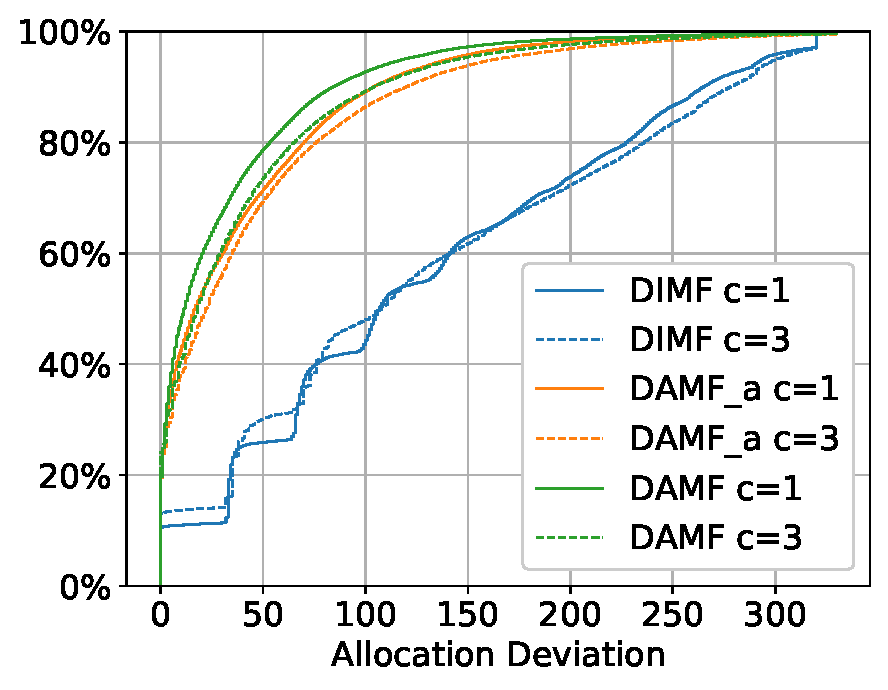
\includegraphics[width=0.24\textwidth]{Image/AD_Ali2017test_Alpha=2.0_40.eps}%
% %\label{fig_second_case}
% \label{Fg:AD_Ali_40}
% }
% \hfil
% \subfloat[Alibaba, workload = 60\%]
% %
% {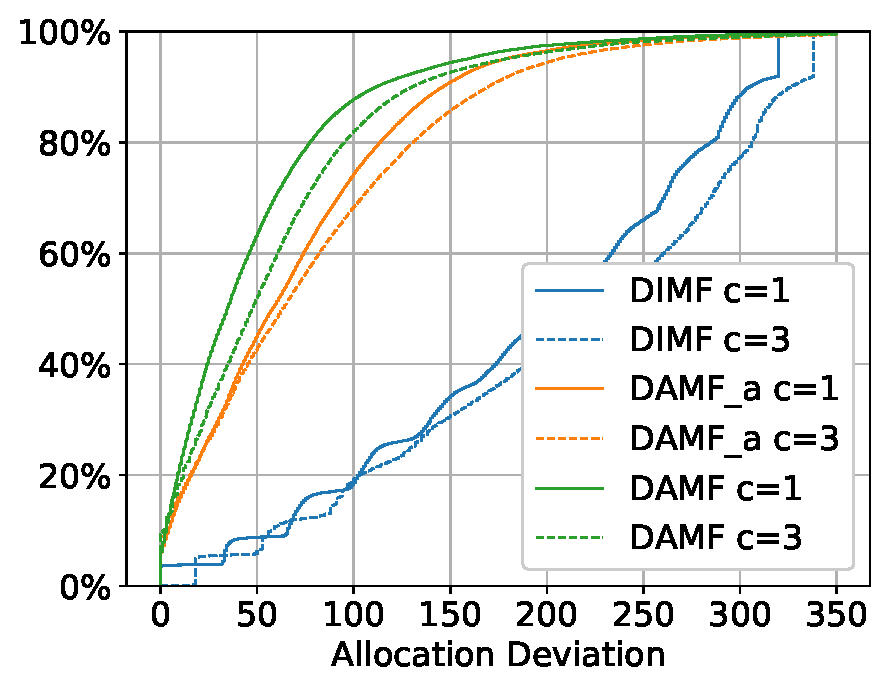
\includegraphics[width=0.24\textwidth]{Image/AD_Ali2017test_Alpha=2.0_60.eps}%
% \label{Fg:AD_Ali_60}
% }
% \hfil
% \subfloat[Google, workload = 40\%]
% %\label{Fg:eg3}
% {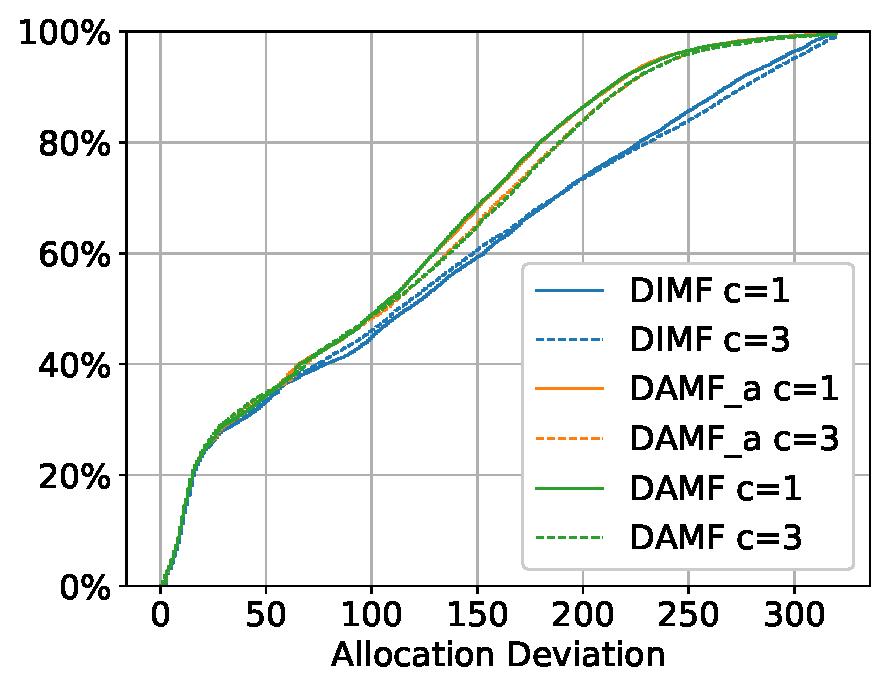
\includegraphics[width=0.24\textwidth]{Image/AD_Gg2019_11_Alpha=2.0_40.eps}%
% \label{Fg:AD_Gg_40}
% }
% \hfil
% \subfloat[Google, workload = 60\%]
% %\label{Fg:eg3}
% {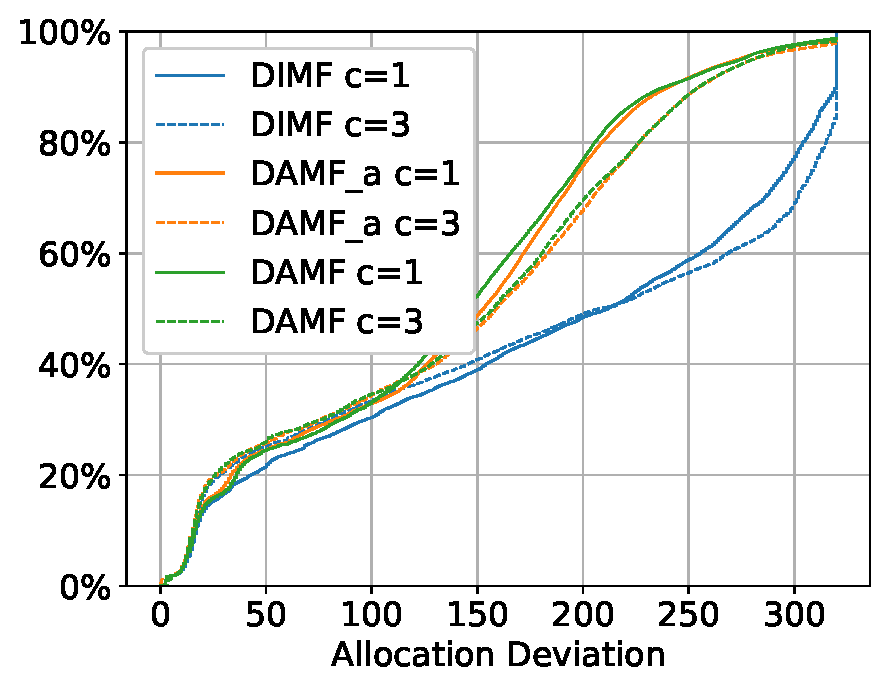
\includegraphics[width=0.24\textwidth]{Image/AD_Gg2019_11_Alpha=2.0_60.eps}%
% \label{Fg:AD_Gg_60}
% }
% \caption{Cumulative distribution of allocation deviation, Zipf parameter $\alpha = 2$}
% \label{fig:AD_instant}
% \end{figure*}

\begin{figure*}[t]
\centering
\subfloat[Alibaba, workload = 40\%]{
    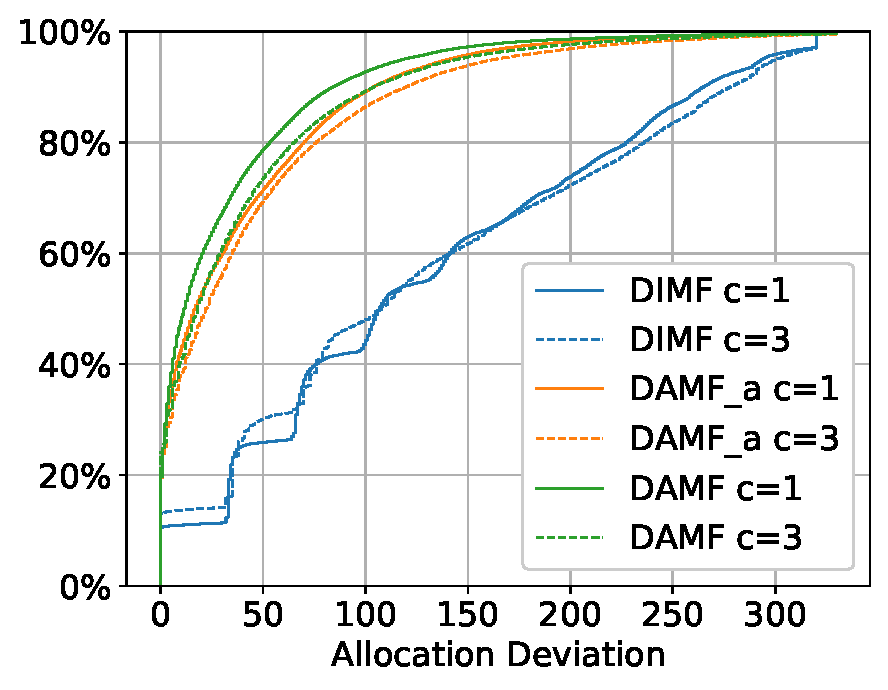
\includegraphics[width=0.47\textwidth]{Image/AD_Ali2017test_Alpha=2.0_40.eps}
    \label{Fg:AD_Ali_40}
}
\hfill
\subfloat[Alibaba, workload = 60\%]{
    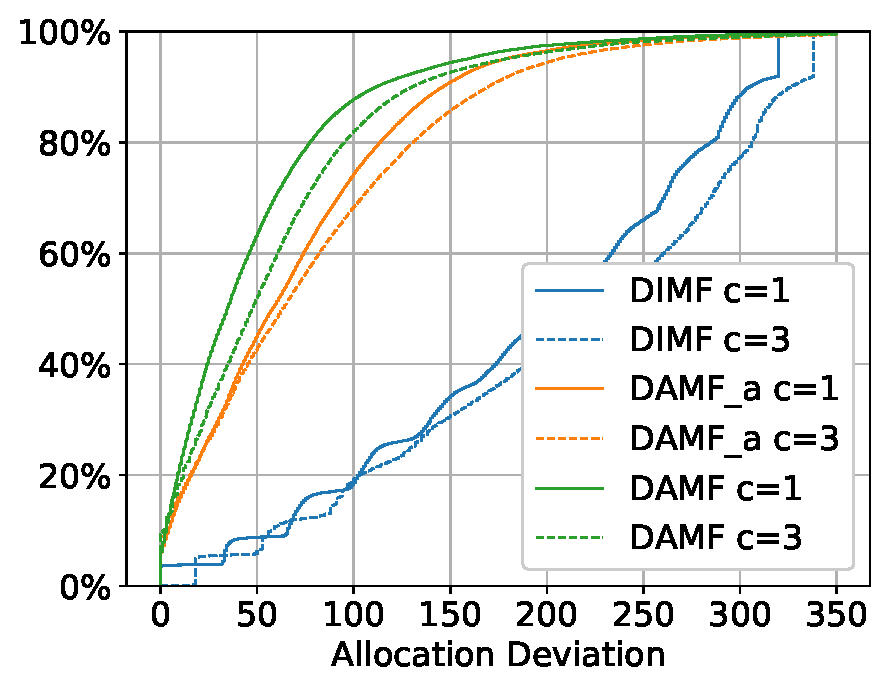
\includegraphics[width=0.47\textwidth]{Image/AD_Ali2017test_Alpha=2.0_60.eps}
    \label{Fg:AD_Ali_60}
}
\vspace{0.8em}
\subfloat[Google, workload = 40\%]{
    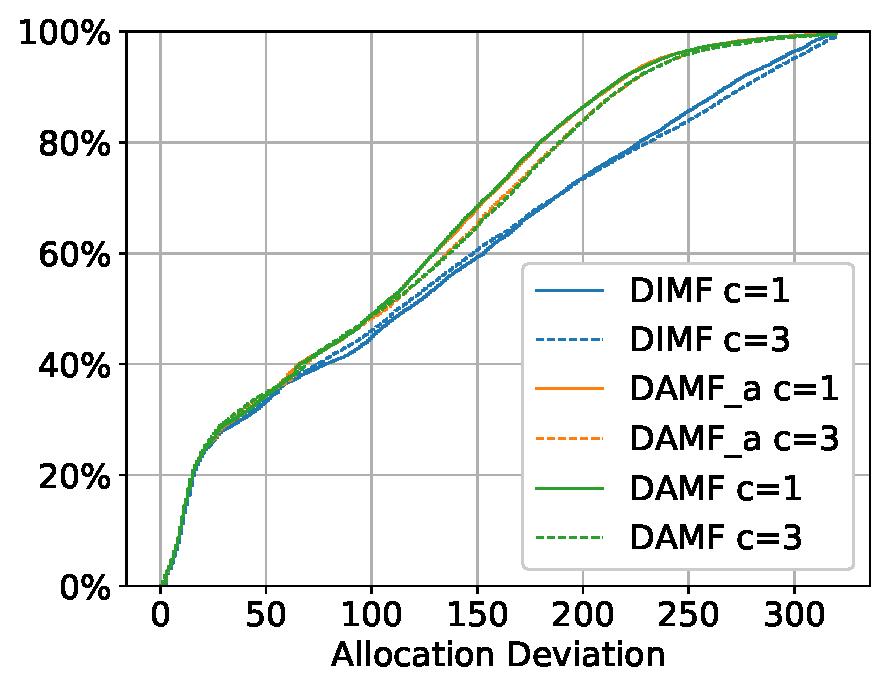
\includegraphics[width=0.47\textwidth]{Image/AD_Gg2019_11_Alpha=2.0_40.eps}
    \label{Fg:AD_Gg_40}
}
\hfill
\subfloat[Google, workload = 60\%]{
    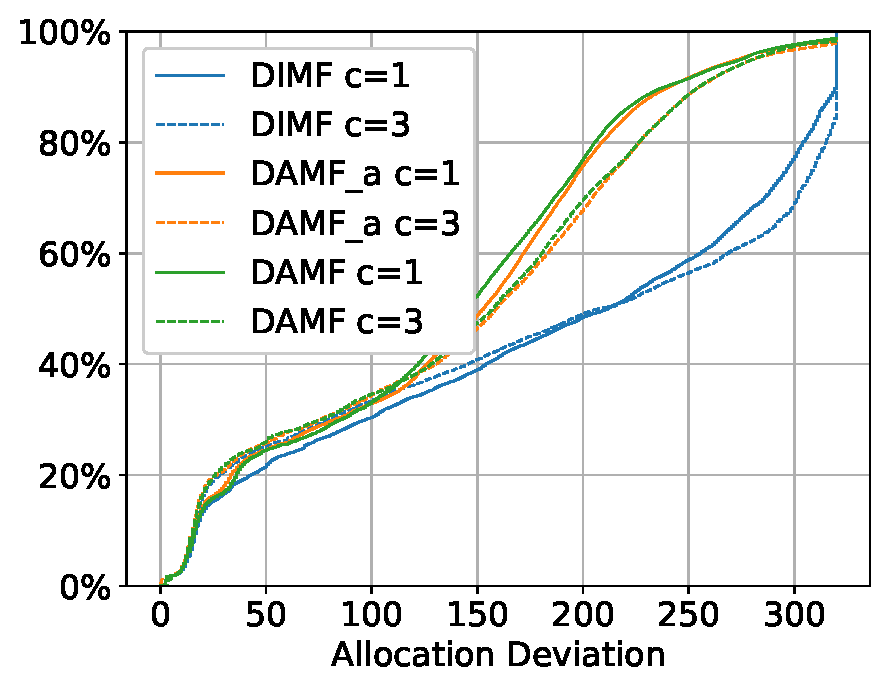
\includegraphics[width=0.47\textwidth]{Image/AD_Gg2019_11_Alpha=2.0_60.eps}
    \label{Fg:AD_Gg_60}
}
\caption{Cumulative distribution of allocation deviation, Zipf parameter $\alpha = 2$.}
\label{fig:AD_instant}
\end{figure*}


\begin{figure*}[t]
\centering
\subfloat[Alibaba, workload = 40\%]
{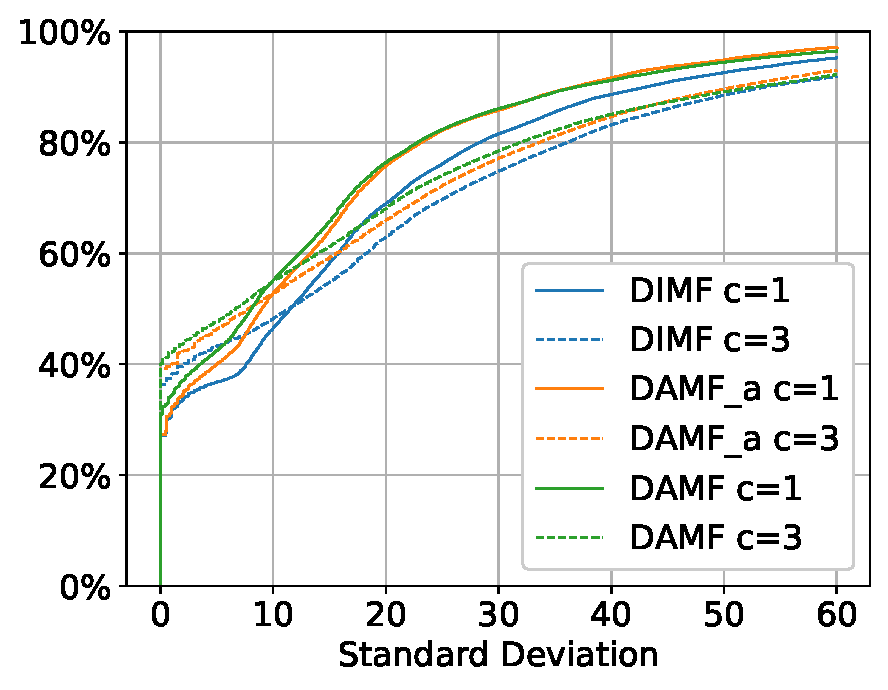
\includegraphics[width=0.48\textwidth]{Image/SD_Ali2017test_Alpha=2.0_40.eps}%
%\label{fig_second_case}
\label{Fg:SD_Ali_40}
}
\vspace{0.8em}
\subfloat[Alibaba, workload = 60\%]
%
{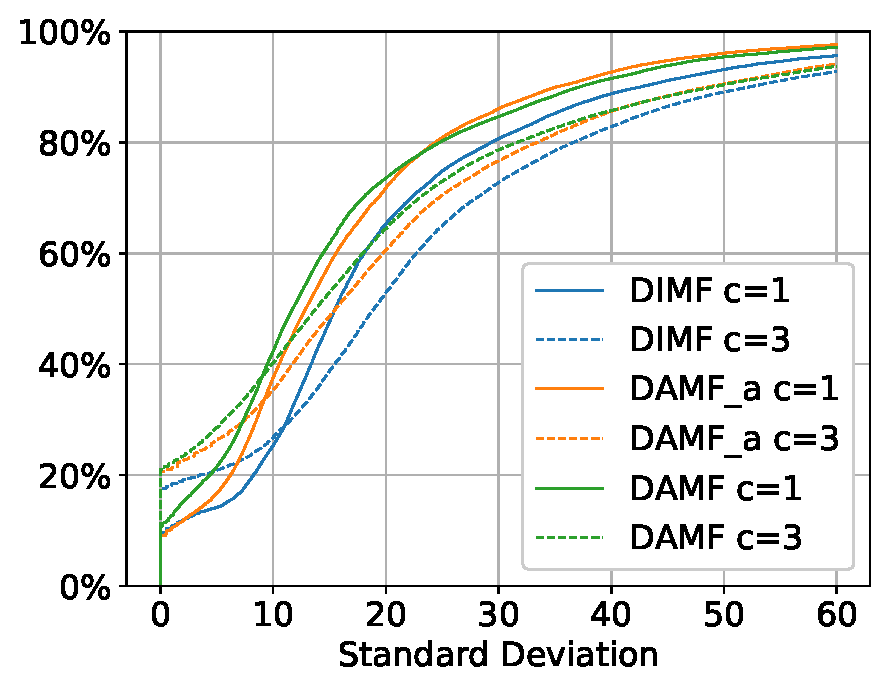
\includegraphics[width=0.48\textwidth]{Image/SD_Ali2017test_Alpha=2.0_60.eps}%
\label{Fg:SD_Ali_60}
}
\hfil
\subfloat[Google, workload = 40\%]
%\label{Fg:eg3}
{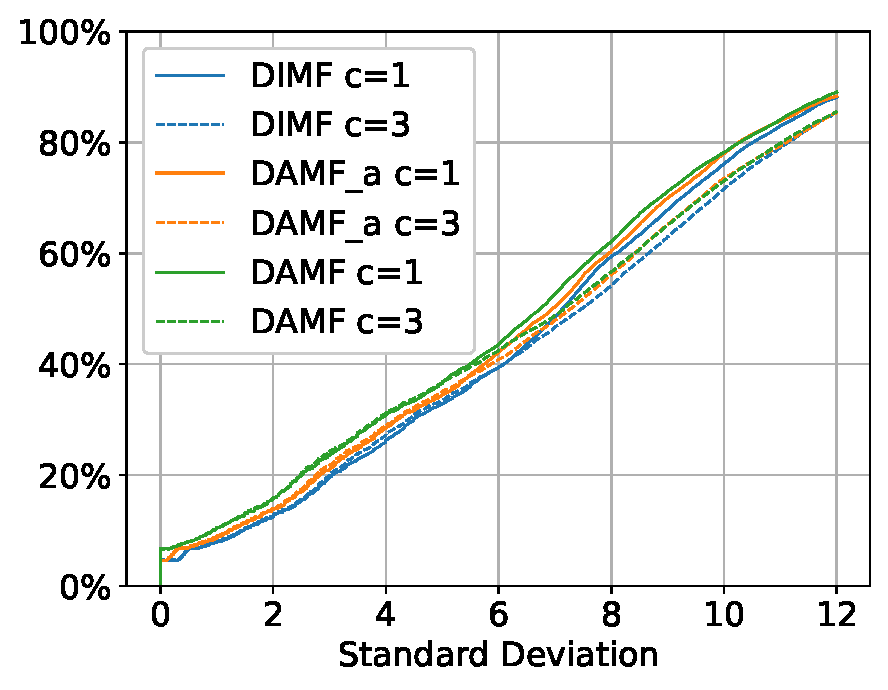
\includegraphics[width=0.48\textwidth]{Image/SD_Gg2019_11_Alpha=2.0_40.eps}%
\label{Fg:SD_Gg_40}
}
\hfil
\subfloat[Google, workload = 60\%]
%\label{Fg:eg3}
{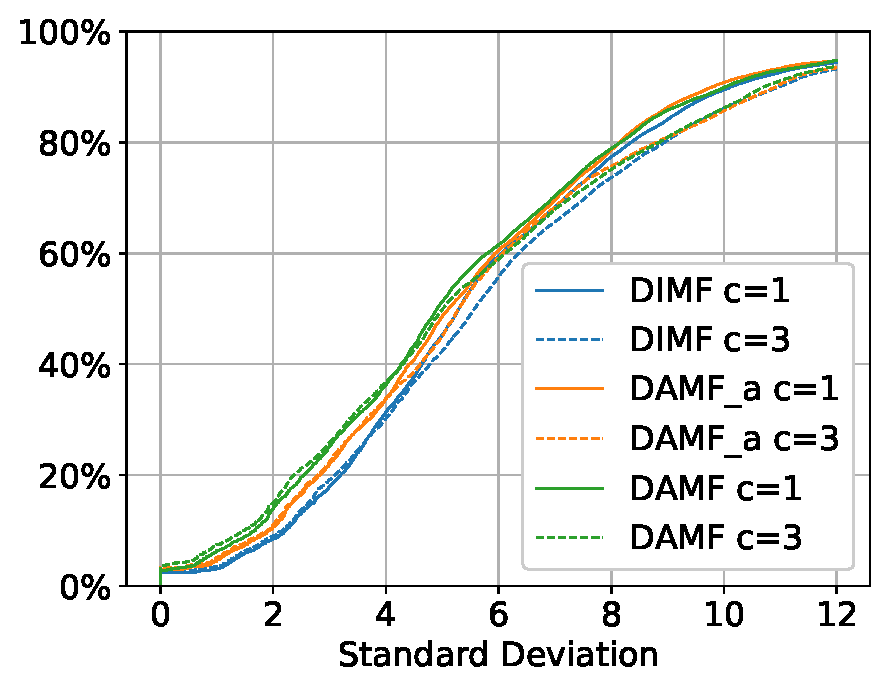
\includegraphics[width=0.48\textwidth]{Image/SD_Gg2019_11_Alpha=2.0_60.eps}%
\label{Fg:SD_Gg_60}
}
\caption{Cumulative distribution of standard deviation, Zipf parameter $\alpha = 2$}
\label{fig:SD_instant}
\end{figure*}

\begin{figure*}[htbp]
\centering
\subfloat[Alibaba, workload = 40\%]
{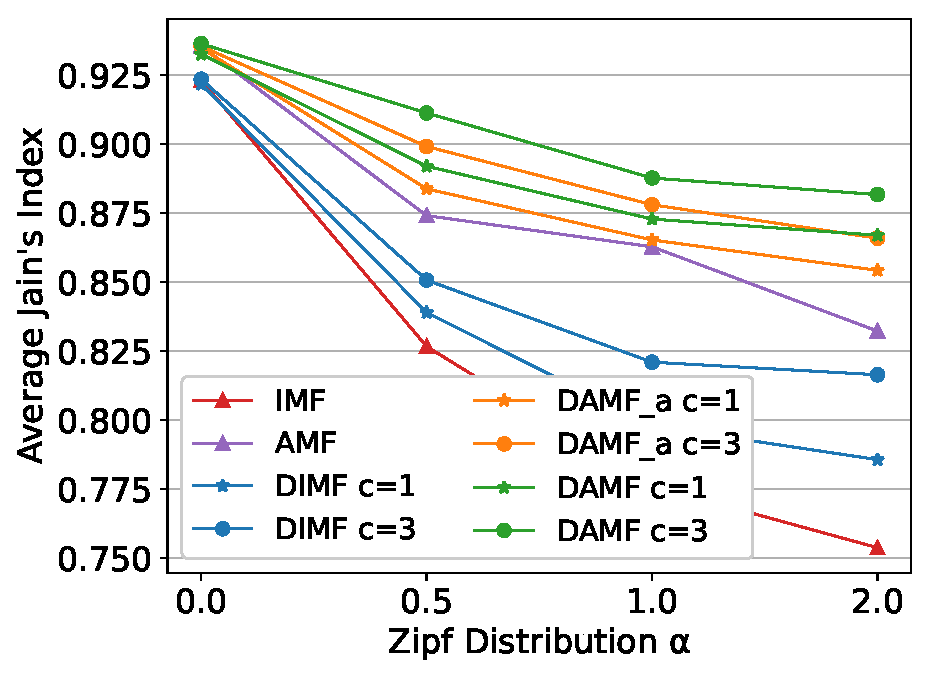
\includegraphics[width=0.48\textwidth]{Image/Jains_Ali2017test_40.eps}%
%\label{fig_second_case}
\label{Fg:Jains_Ali_40}
}
\hfil
\subfloat[Alibaba, workload = 60\%]
%
{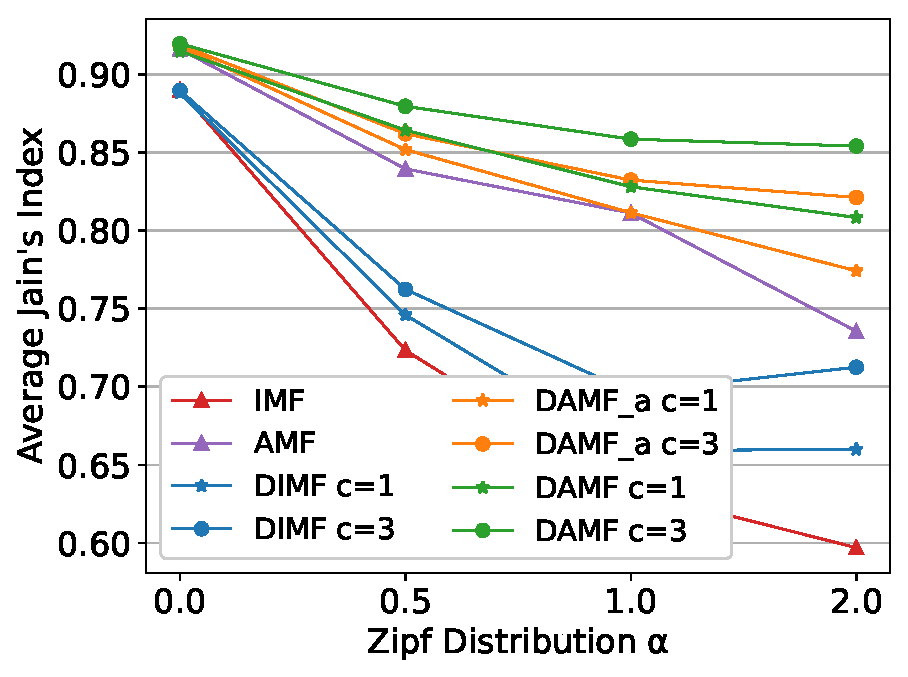
\includegraphics[width=0.48\textwidth]{Image/Jains_Ali2017test_60.eps}%
\label{Fg:Jains_Ali_60}
}
\vspace{0.8em}
\subfloat[Google, workload = 40\%]
%\label{Fg:eg3}
{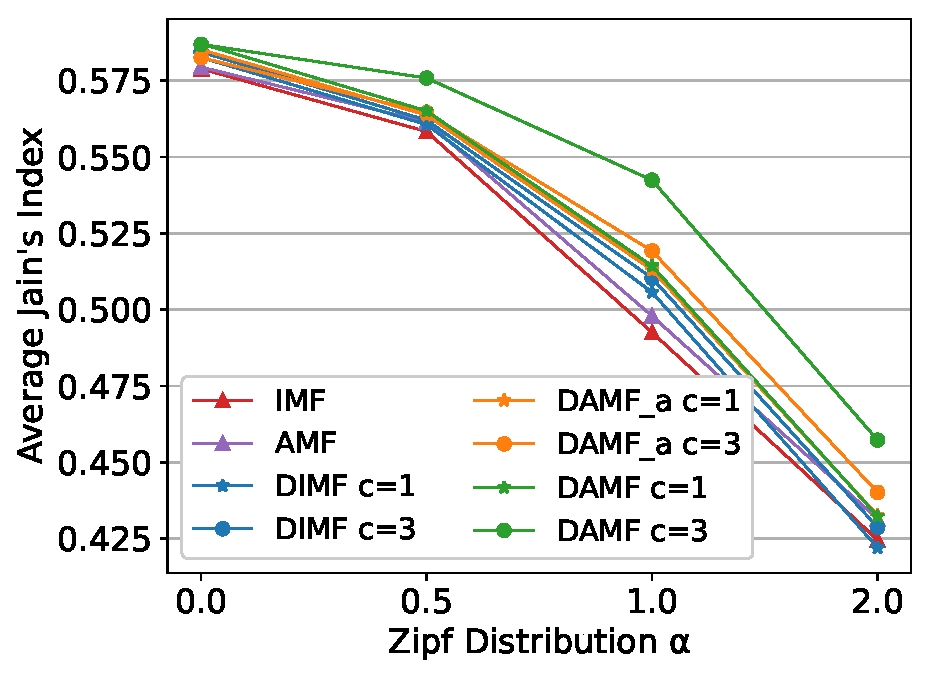
\includegraphics[width=0.48\textwidth]{Image/Jains_Gg2019_11_40.eps}%
\label{Fg:Jains_Gg_40}
}
\hfil
\subfloat[Google, workload = 60\%]
%\label{Fg:eg3}
{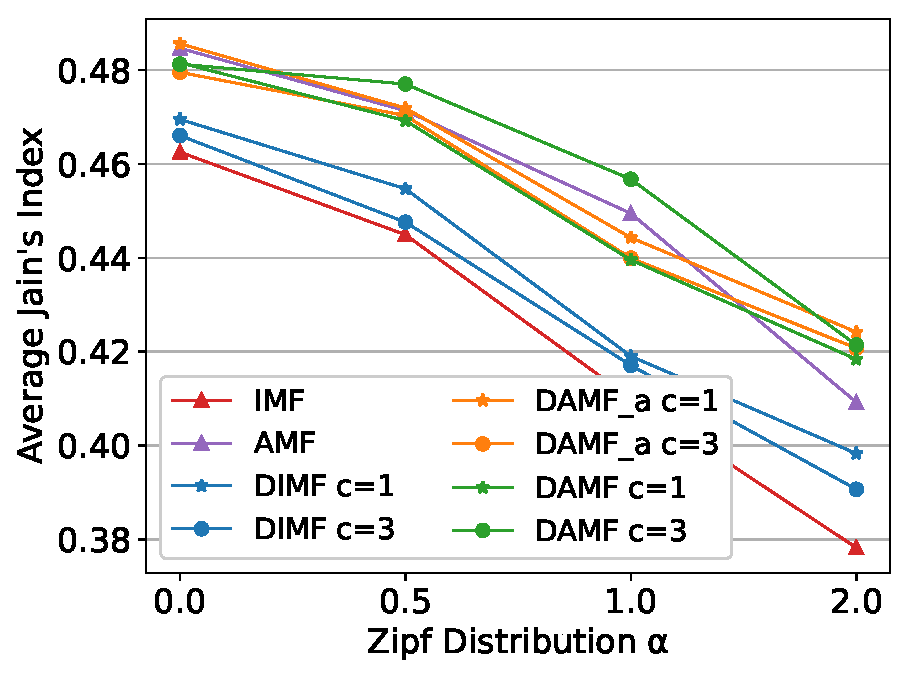
\includegraphics[width=0.48\textwidth]{Image/Jains_Gg2019_11_60.eps}%
\label{Fg:Jains_Gg_60}
}
\caption{Average Jain's Index}
\label{fig:Average Jain's Index}
\end{figure*}

\begin{figure*}[t]
\centering
\subfloat[Alibaba, workload = 40\%]
{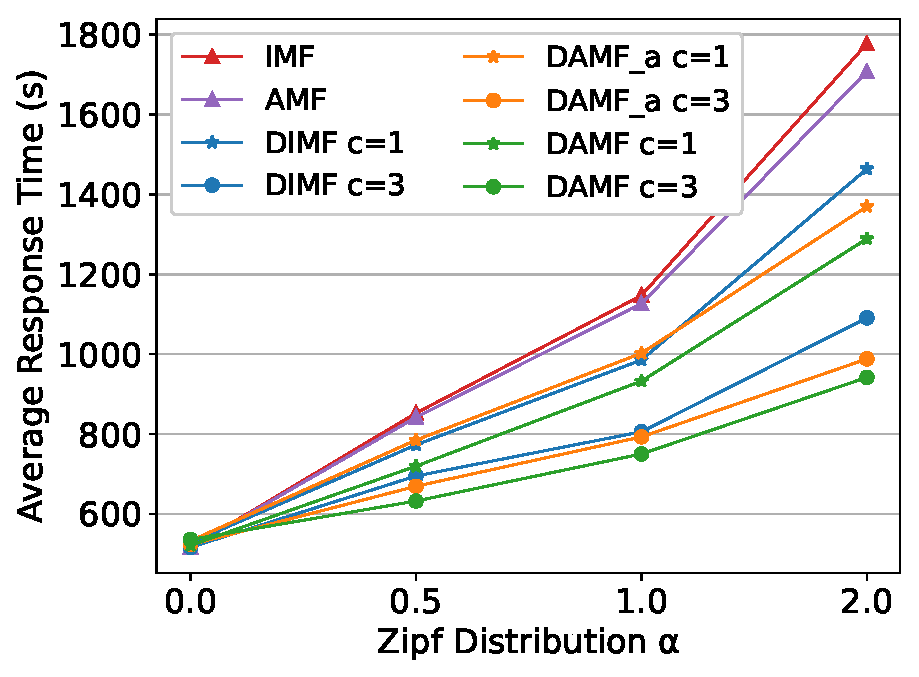
\includegraphics[width=0.48\textwidth]{Image/Workload_Ali2017test_40.eps}%
%\label{fig_second_case}
\label{Fg:JRT_Ali_40}
}
\hfil
\subfloat[Alibaba, workload = 60\%]
%
{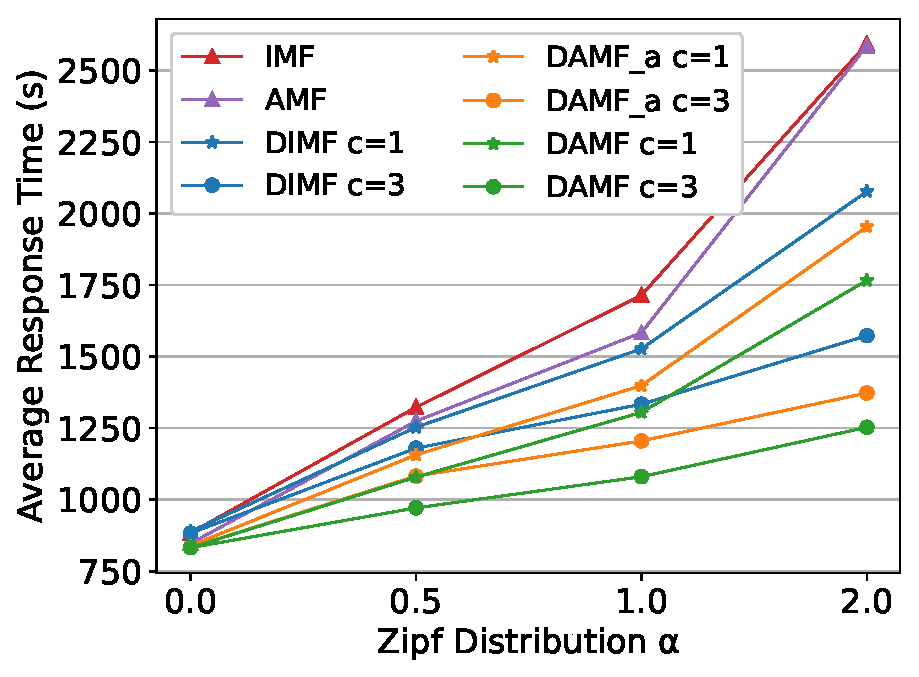
\includegraphics[width=0.48\textwidth]{Image/Workload_Ali2017test_60.eps}%
\label{Fg:JRT_Ali_60}
}
\vspace{0.8em}
\subfloat[Google, workload = 40\%]
%\label{Fg:eg3}
{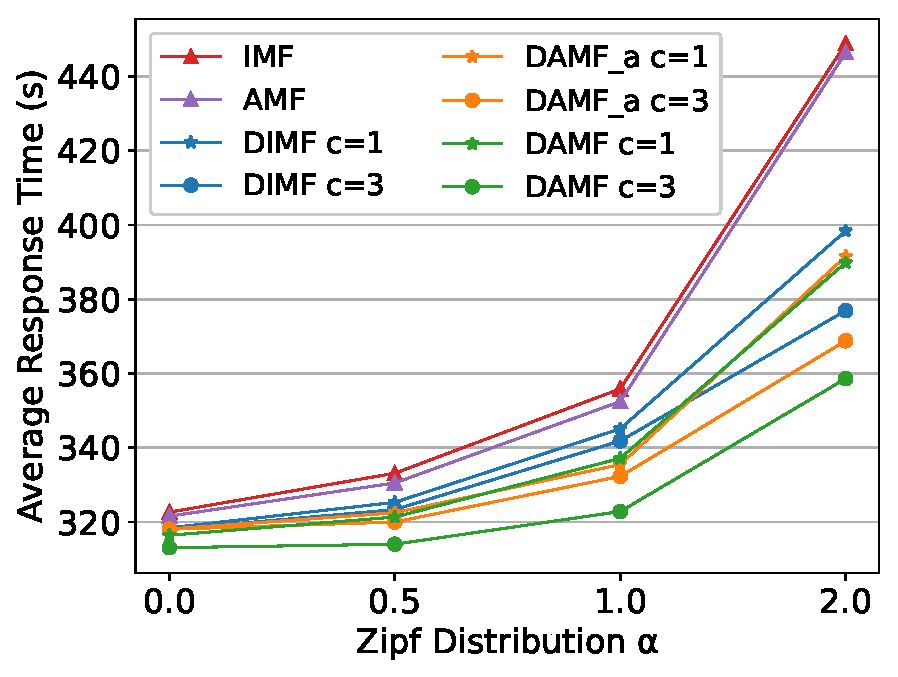
\includegraphics[width=0.48\textwidth]{Image/Workload_Gg2019_11_40.eps}%
\label{Fg:JRT_Gg_40}
}
\hfil
\subfloat[Google, workload = 60\%]
%\label{Fg:eg3}
{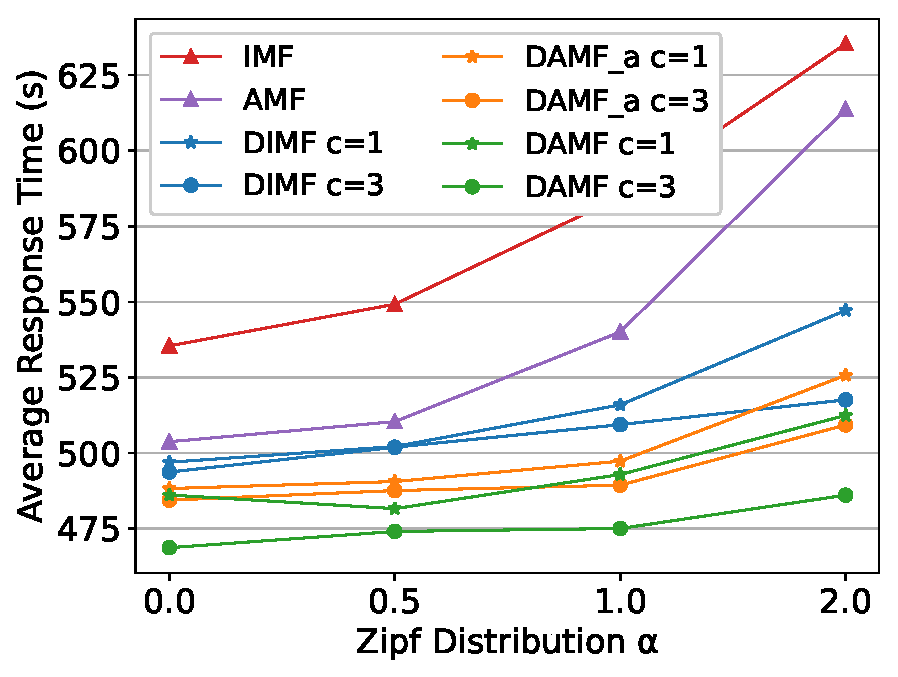
\includegraphics[width=0.48\textwidth]{Image/Workload_Gg2019_11_60.eps}%
\label{Fg:JRT_Gg_60}
}
\caption{Average job response time}
\label{fig:Average Response Time}
\end{figure*}

The response time of a job is the time duration from its arrival to its completion. We use the average job response time to evaluate the long-term impact of allocation policies. A lower average job response time suggests a higher system efficiency. 

\subsection{Experimental Results}

\begin{table}[t]
  \caption{Average computation time (s), Alibaba}
  \label{tab:computation_time_ali}
  \centering
    \begin{tabularx}{0.65\textwidth}{cccccc}
      \toprule
      & & \multicolumn{2}{c}{workload = 40\%} & \multicolumn{2}{c}{workload = 60\%} \\
      \midrule
      $c$ & $\alpha$ & DAMF & DAMF\_a & DAMF & DAMF\_a \\
      \midrule
      \multirow{4}{*}{1} 
      & 0.0 & $0.0747$ & $1.005*10^{-5}$ &  $0.1287$ & $1.402*10^{-5}$\\
      & 0.5 & $0.0792$ & $9.223*10^{-6}$&  $0.1661$ & $1.440*10^{-5}$\\
      & 1.0 & $0.0793$ & $9.409*10^{-6}$&  $0.1764$ & $1.453*10^{-5}$\\
      & 2.0 & $0.0841$ & $8.205*10^{-6}$&  $0.1709$ & $1.401*10^{-5}$\\
      \midrule
      \multirow{4}{*}{3} 
      & 0.0 & $0.0709$ & $8.749*10^{-6}$&  $0.1497$ & $1.690*10^{-5}$ \\
      & 0.5 & $0.0765$ & $8.395*10^{-6}$& $0.1571$ & $1.351*10^{-5}$ \\
      & 1.0 & $0.0761$ & $8.853*10^{-6}$& $0.1551$ & $1.424*10^{-5}$ \\
      & 2.0 & $0.0837$ & $1.051*10^{-5}$& $0.1733$ & $1.316*10^{-5}$ \\
      \bottomrule
    \end{tabularx}
\end{table}

\begin{table}[t]
  \caption{Average computation time (s), Google}
  \label{tab:computation_time_gg}
  \centering
    \begin{tabularx}{0.65\textwidth}{cccccc}
      \toprule
      & & \multicolumn{2}{c}{workload = 40\%} & \multicolumn{2}{c}{workload = 60\%}\\
      \midrule
      $c$ & $\alpha$ & DAMF & DAMF\_a & DAMF & DAMF\_a\\
      \midrule
      \multirow{4}{*}{1} 
      & 0.0 & $0.1029$ & $1.710*10^{-5}$ &$0.3783$ & $6.346*10^{-5}$ \\
      & 0.5 & $0.1247$ & $1.836*10^{-5}$ &$0.3771$ & $6.084*10^{-5}$ \\
      & 1.0 & $0.1298$ & $1.610*10^{-5}$&$0.3952$ & $5.071*10^{-5}$ \\
      & 2.0 & $0.1164$ & $1.686*10^{-5}$&$0.3708$ & $3.817*10^{-5}$ \\
      \midrule
      \multirow{4}{*}{3} 
      & 0.0 & $0.1180$ & $1.508*10^{-5}$&$0.4670$ & $7.205*10^{-5}$ \\
      & 0.5 & $0.1400$ & $1.583*10^{-5}$& $0.5175$ & $5.482*10^{-5}$ \\
      & 1.0 & $0.1489$ & $1.496*10^{-5}$& $0.5289$ & $5.178*10^{-5}$ \\
      & 2.0 &  $0.1796$ & $1.798*10^{-5}$ & $0.5465$ & $3.670*10^{-5}$ \\
      \bottomrule
    \end{tabularx}
\end{table}

Figure \ref{fig:AD_instant} shows the cumulative distribution of the allocation deviation from the ideal DAMF. Due to space limitations, we only present the results for the Zipf distribution of $\alpha = 2$. The results for other Zipf distributions show similar trends. Comparing DAMF and the baseline DIMF under the same transfer limit, it can be seen that DAMF's distribution curves are closer to the upper left corner, which indicates that DAMF achieves better instantaneous fairness than DIMF. In addition, the distribution curves of DAMF and DAMF\_a are rather close to each other under the same transfer limit, demonstrating that DAMF\_a is a close approximation of DAMF. We also record and compare the average computation time for recomputing allocation matrices during simulations. As shown in Table \ref{tab:computation_time_ali} and \ref{tab:computation_time_gg}, DAMF\_a reduces the average computation time by four orders of magnitude compared to DAMF (from the order of $10^{-1}$ seconds down to $10^{-5}$ seconds).

Comparing the results for the Alibaba and Google datasets under the same transfer limit, it can be seen that the Google dataset has much higher allocation deviations than the Alibaba dataset. This is mainly due to task durations: the Google dataset has much longer task durations than the Alibaba dataset as shown in Table \ref{tab3:data_characteristics}. Since there is no preemption, an updated allocation matrix after recomputation starts to take effect only after the computing slots are released (when the currently running tasks are completed) and reallocated to the intended jobs. Longer task durations make it slower for the actual allocation to converge to the allocation matrix computed.

Figure \ref{fig:SD_instant} shows the cumulative distribution of the standard deviation of the instantaneous resource allocation among jobs. Due to space limitations, we again only present the results for the Zipf distribution of $\alpha = 2$. Similar to the results in Figure \ref{fig:AD_instant}, it can be seen that DAMF’s distribution curves are closer to the upper left corner, which indicates that DAMF achieves more balanced instantaneous resource allocations than DIMF. Comparing DAMF and DAMF\_a under the same transfer limit, we can see that their distribution curves are quite close to each other, which again shows that DAMF\_a is a close approximation of DAMF. It can also be observed from Figure \ref{fig:SD_instant} that the standard deviation tends to increase with the transfer limit. This is because in DAMF, small-demand jobs are prioritized to have their demands fully satisfied at their original sites, while large-demand jobs are more likely to have unsatisfied demands and tend to exploit idle compute resources at other sites by leveraging network resources. Therefore, transmissions often help large-demand jobs to obtain more resources while keeping the resources allocated to small-demand jobs unchanged, which leads to the rise of the standard deviation of the instantaneous resource allocation with increasing transfer limit.

Figure \ref{fig:Average Jain's Index} shows the average Jain's Index. It can be seen that allocation policies that allow task transmissions (DAMF, DAMF\_a, DIMF) have higher Jain's Indexes compared with their counterparts which do not (AMF, IMF). More importantly, DAMF achieves the highest index while DAMF\_a is close to it, demonstrating that they effectively reduce the imbalance of resource allocation among jobs.

Figure \ref{fig:Average Response Time} shows the average job response time for different datasets, system workloads and Zipf distributions. It can be seen that policies utilizing network resources achieve lower average job response time, compared with IMF and AMF. The improvement typically increases with the transfer limit. Furthermore, since DAMF views the whole distributed system as a united resource pool and requires the aggregate allocation vector to be max-min fair among all possible transmissions and allocations, it outperforms DIMF and other allocation policies in most cases. The improvement is substantial even with only one bandwidth unit available, and it becomes more significant when the system workload is higher or the task distribution of jobs is more skewed among sites. In addition, DAMF\_a has similar performance of average job response time to DAMF, demonstrating that it closely approximates the original DAMF.

\subsection{Evaluation on Robustness and Scalability}

\begin{figure*}[t]
\centering
\subfloat[Alibaba, workload = 40\%]
{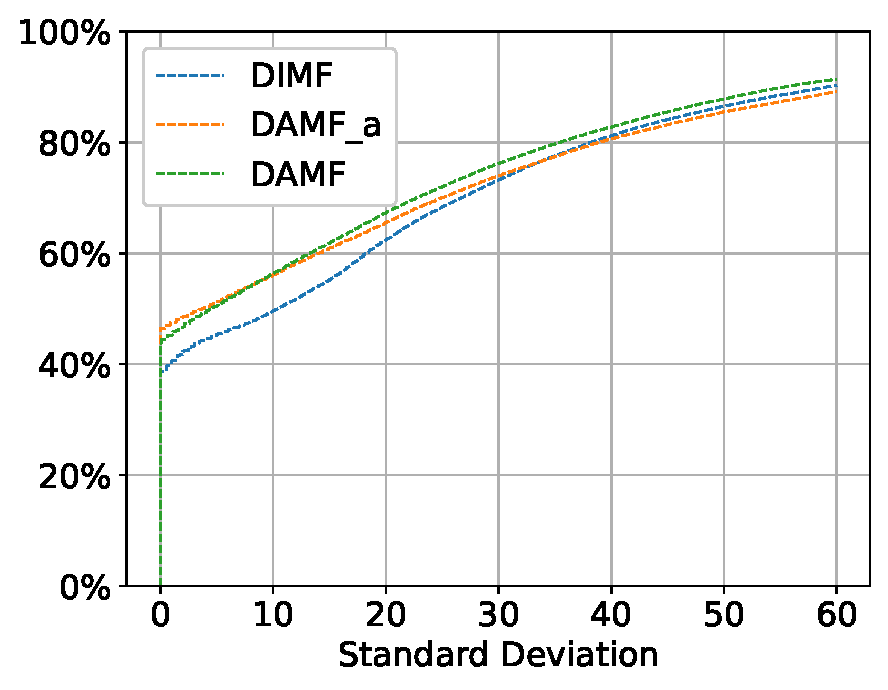
\includegraphics[width=0.48\textwidth]{Image/SD_Ali2017test_Alpha=2.0_40f.eps}
\label{Fg:SD_Ali_40f}
}
\hfil
\subfloat[Alibaba, workload = 60\%]
%
{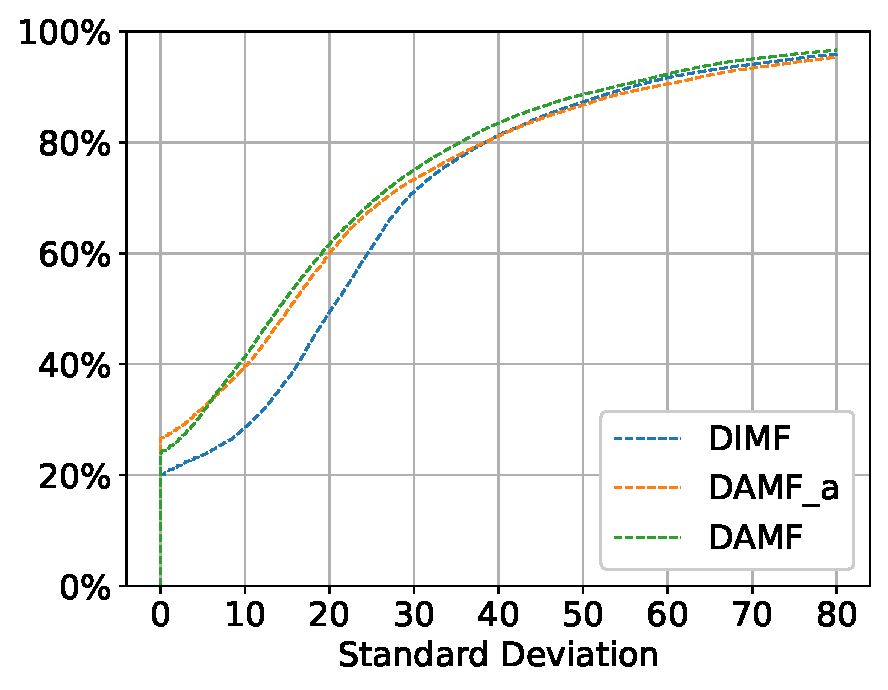
\includegraphics[width=0.48\textwidth]{Image/SD_Ali2017test_Alpha=2.0_60f.eps}%
\label{Fg:SD_Ali_60f}
}
\vspace{0.8em}
\subfloat[Google, workload = 40\%]
%
{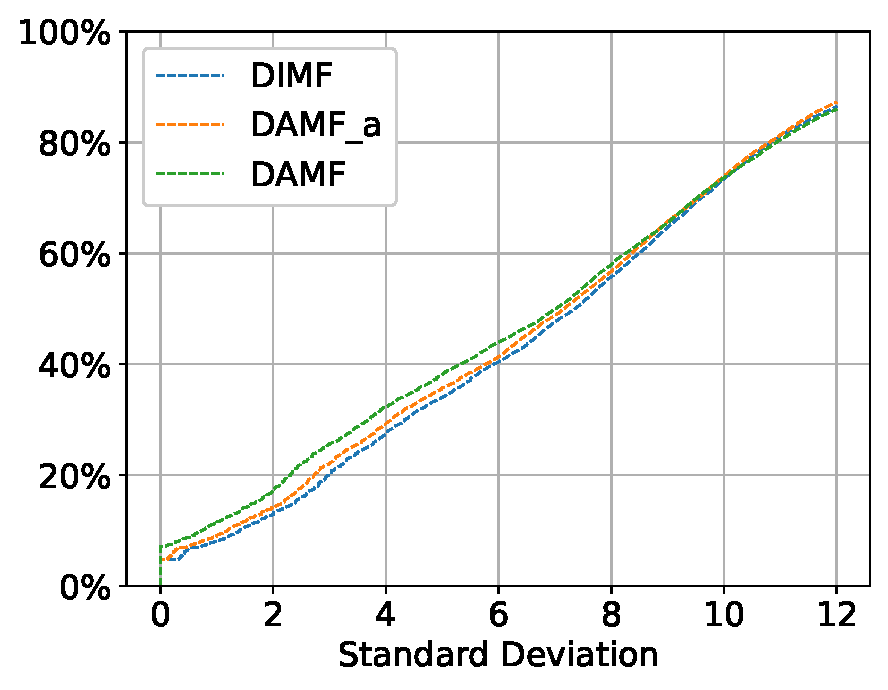
\includegraphics[width=0.48\textwidth]{Image/SD_Gg2019_11_Alpha=2.0_40f.eps}%
\label{Fg:SD_Gg_40f}
}
\hfil
\subfloat[Google, workload = 60\%]
%
{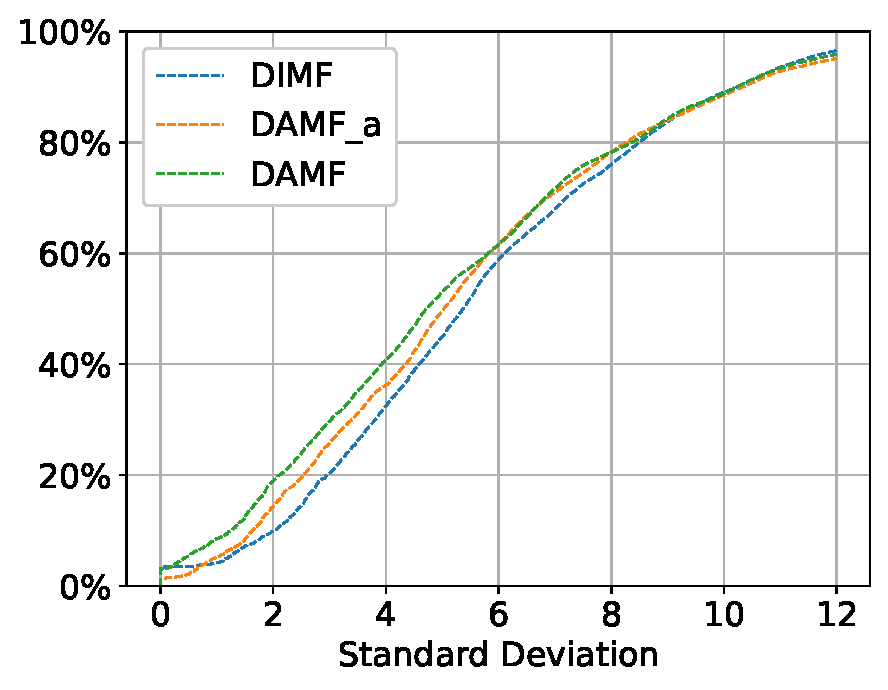
\includegraphics[width=0.48\textwidth]{Image/SD_Gg2019_11_Alpha=2.0_60f.eps}%
\label{Fg:SD_Gg_60f}
}
\caption{Cumulative distribution of standard deviation under fluctuating bandwidth, Zipf parameter $\alpha = 2$}
\label{fig:SD_f}
\end{figure*}

\begin{figure*}[t]
\centering
\subfloat[Alibaba, workload = 40\%]
{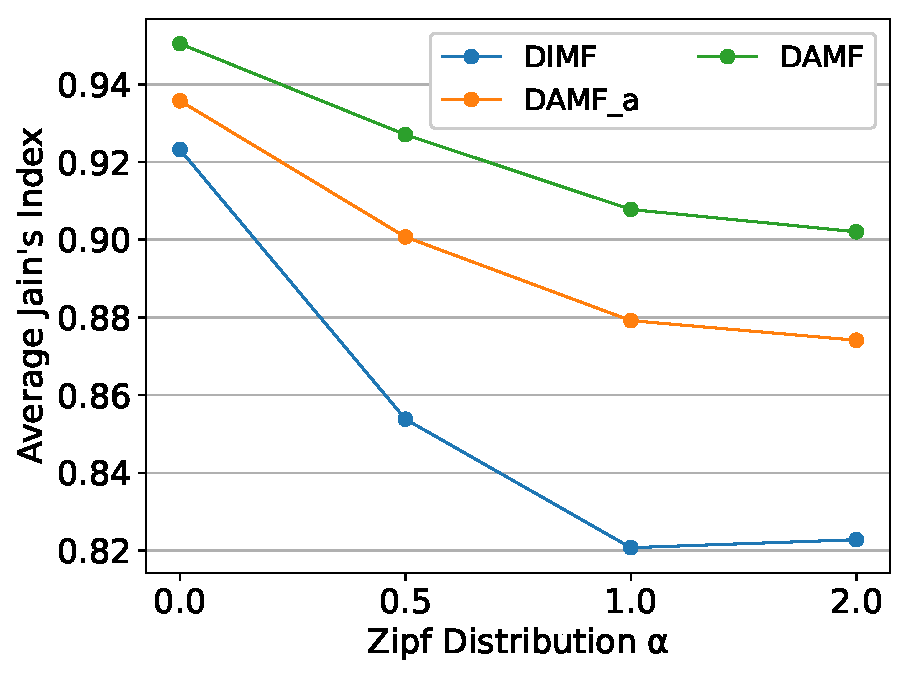
\includegraphics[width=0.48\textwidth]{Image/Jains_Ali2017test_40f.eps}%
\label{Fg:Jains_Ali_40f}
}
\hfil
\subfloat[Alibaba, workload = 60\%]
%
{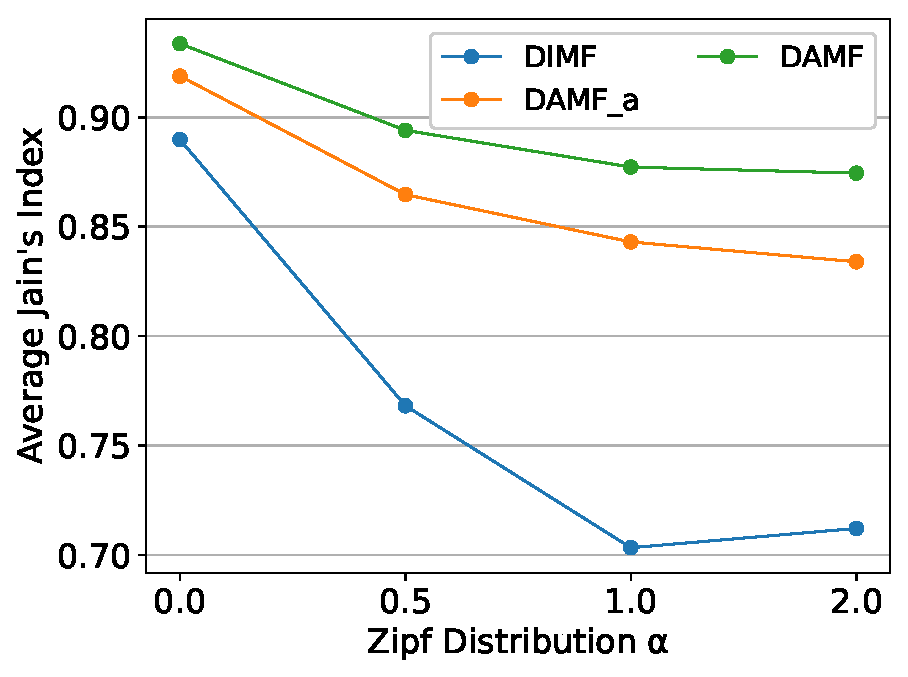
\includegraphics[width=0.48\textwidth]{Image/Jains_Ali2017test_60f.eps}%
\label{Fg:Jains_Ali_60f}
}
\vspace{0.8em}
\subfloat[Google, workload = 40\%]
%
{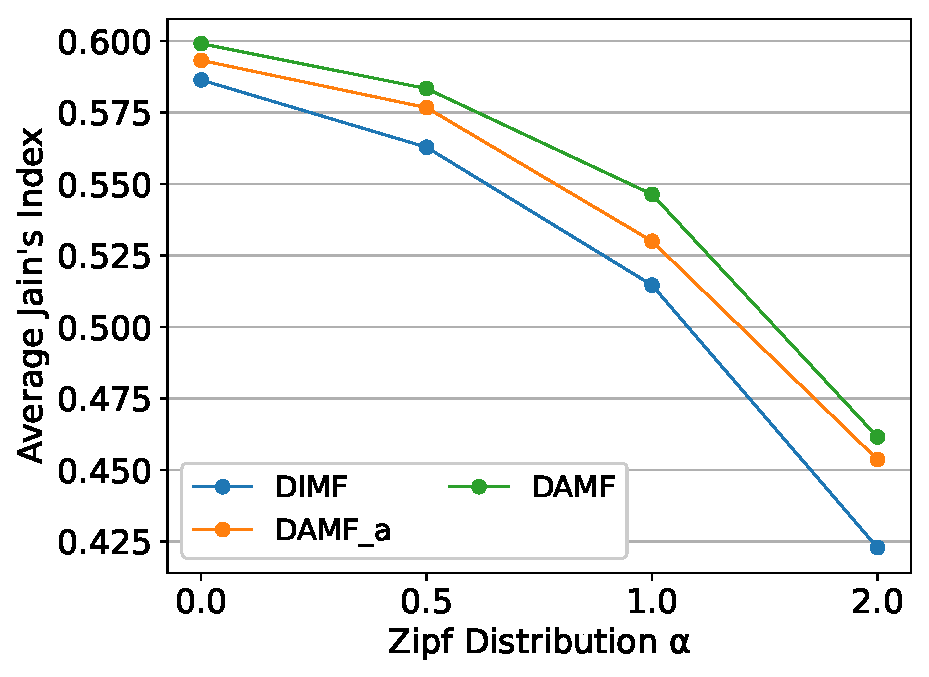
\includegraphics[width=0.48\textwidth]{Image/Jains_Gg2019_11_40f.eps}%
\label{Fg:Jains_Gg_40f}
}
\hfil
\subfloat[Google, workload = 60\%]
%
{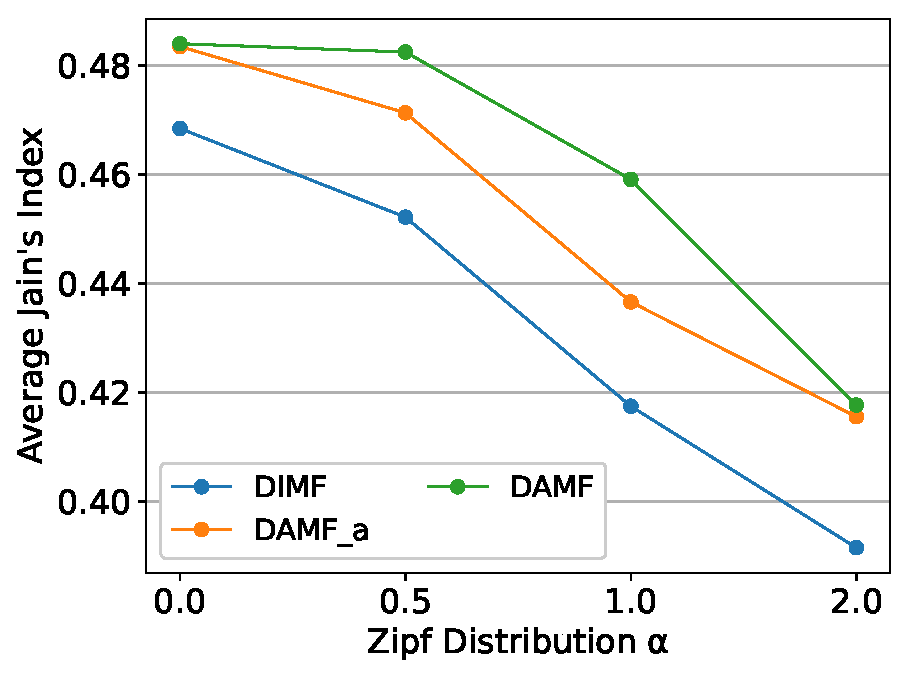
\includegraphics[width=0.48\textwidth]{Image/Jains_Gg2019_11_60f.eps}%
\label{Fg:Jains_Gg_60f}
}
\caption{Average Jain's Index under fluctuating bandwidth}
\label{fig:Average Jain's_f}
\end{figure*}

\begin{figure*}[t]
\centering
\subfloat[Alibaba, workload = 40\%]
{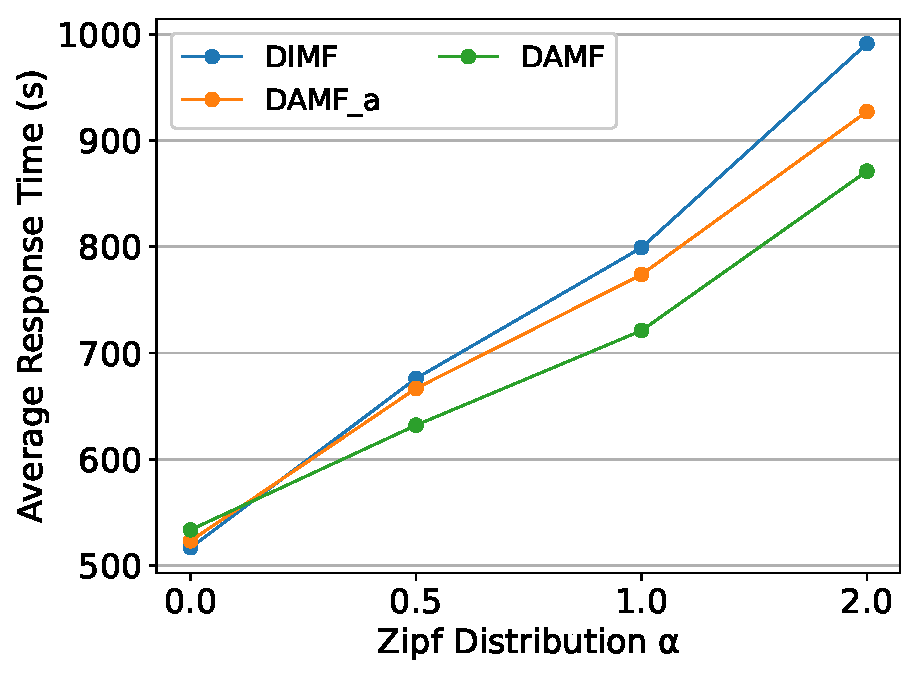
\includegraphics[width=0.48\textwidth]{Image/Workload_Ali2017test_40f.eps}%
\label{Fg:JRT_Ali_40f}
}
\hfil
\subfloat[Alibaba, workload = 60\%]
%
{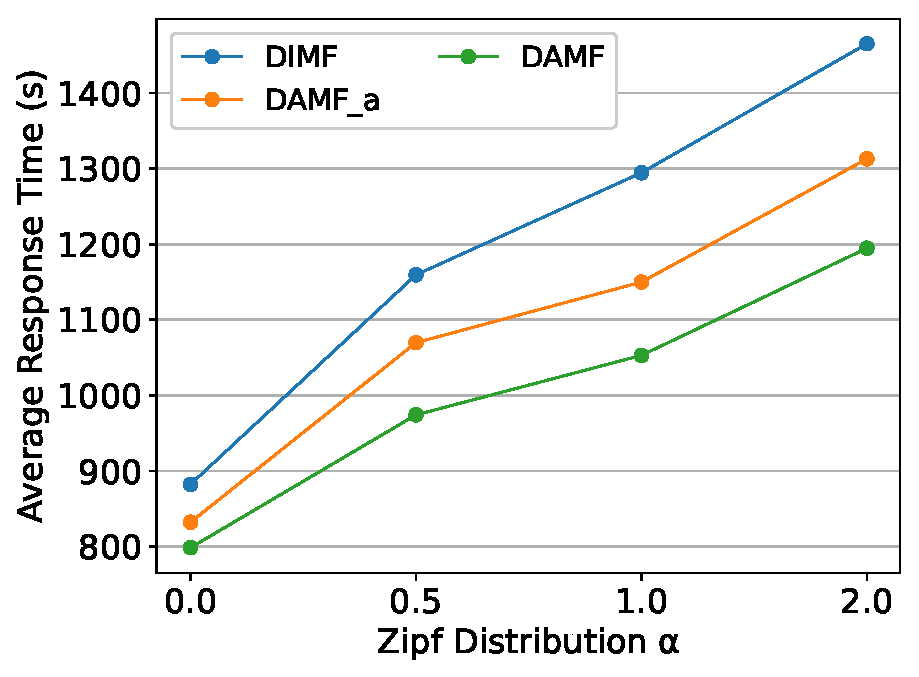
\includegraphics[width=0.48\textwidth]{Image/Workload_Ali2017test_60f.eps}%
\label{Fg:JRT_Ali_60f}
}
\vspace{0.8em}
\subfloat[Google, workload = 40\%]
%
{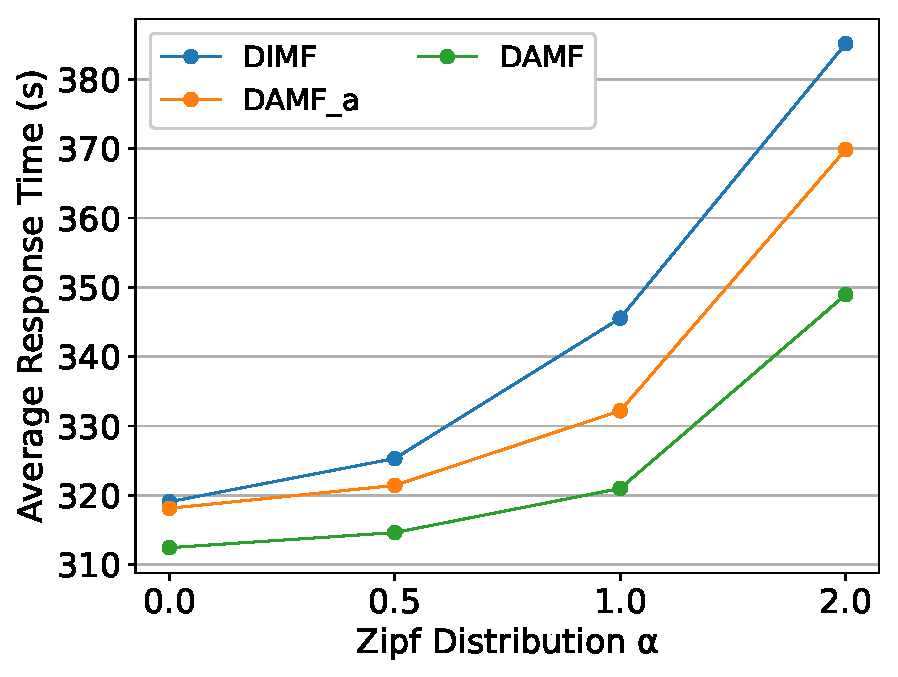
\includegraphics[width=0.48\textwidth]{Image/Workload_Gg2019_11_40f.eps}%
\label{Fg:JRT_Gg_40f}
}
\hfil
\subfloat[Google, workload = 60\%]
%
{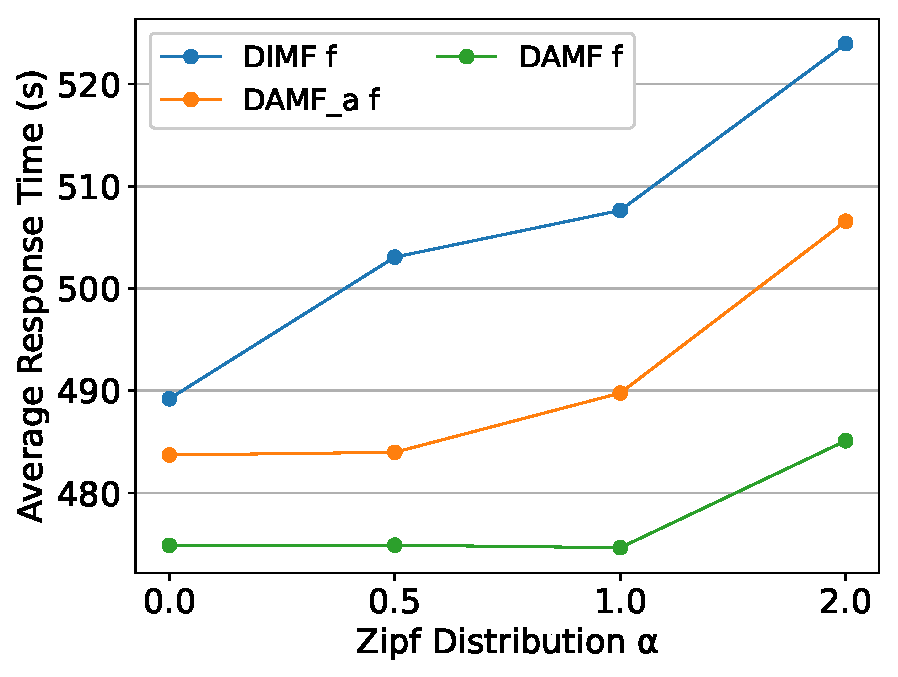
\includegraphics[width=0.48\textwidth]{Image/Workload_Gg2019_11_60f.eps}%
\label{Fg:JRT_Gg_60f}
}
\caption{Average job response time under fluctuating bandwidth}
\label{fig:Average Response Time_f}
\end{figure*}


We also conduct experiments to evaluate the allocation policies under fluctuating bandwidth conditions. Specifically, we initialize an integer sequence randomly generated from a uniform distribution between 1 and 5 to simulate the changes of the transfer count limit $c$ (which reflects the available bandwidth) over time. In the experiments, once the $i$-th job arrives, the value of $c$ for all sites is changed to the $i$-th element in the sequence for recomputation. For fair comparison, the same sequence is used for evaluating all allocation policies. As shown in Figures \ref{fig:SD_f}, \ref{fig:Average Jain's_f} and \ref{fig:Average Response Time_f}, the performance trends of different policies (that utilize network resources) remain similar to previous experiments. DAMF and DAMF\_a again significantly outperform the baseline policy DIMF.

In addition, we evaluate the scalability of DAMF\_a under larger numbers of sites $m$. We set $m=20$, $50$ and $100$ and conduct experiments for DAMF\_a and DIMF. Since the average task count per job of the Google dataset is low (4.5 tasks per job), it is not suitable for evaluation with a large number of sites. Thus, we test with the Alibaba dataset only. Due to space limitations, for performance metrics other than the average computation time, we present only the results for the Zipf distribution of $\alpha=1$ in Figures \ref{fig:SD_sites1}, \ref{fig:SD_sites2}, \ref{fig:Average_Response_Time_sites} and \ref{fig:Jains_sites} (those for other $\alpha$ values show similar trends). These results again demonstrate that DAMF\_a outperforms the baseline DIMF in terms of both resource allocation fairness and system utility. Table \ref{tab:computation_time_m} shows the average computation times for different site numbers and Zipf distributions. These results demonstrate that DAMF\_a maintains low computational overhead, thereby validating its potential for large-scale geo-distributed systems.

\begin{figure*}[t]
\centering
% 子图 1
\begin{subfigure}[b]{0.31\linewidth}
  \centering
  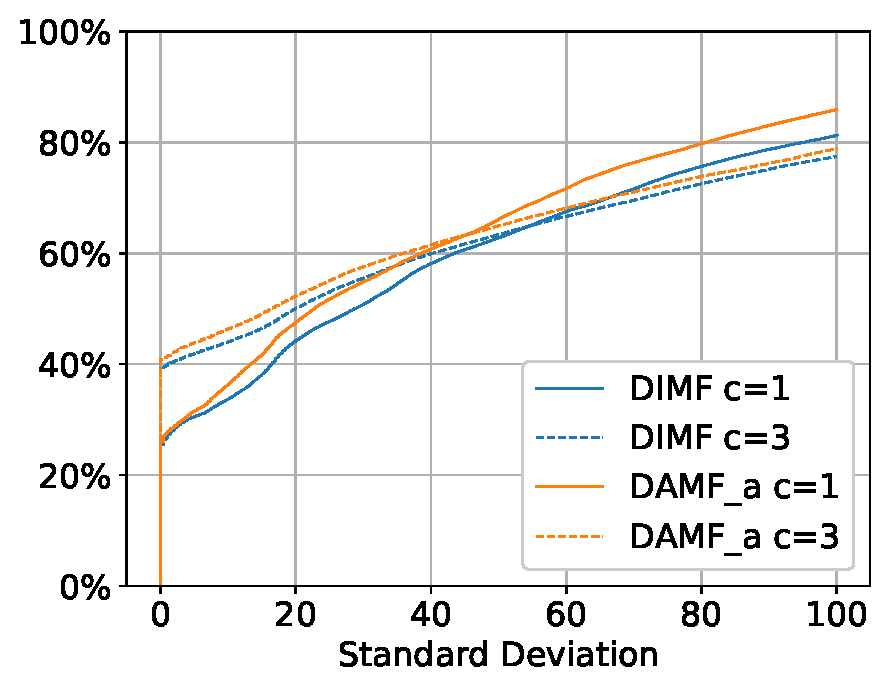
\includegraphics[width=\linewidth]{Image/SD_Ali2017test_Alpha=1.0_40_sites=20.eps}
  \caption{$m=20$}
  \label{Fg:SD_Ali_40_20m}
\end{subfigure}
\hfill % 用 \hfill 代替 \hfil，自动拉开完美的间距
% 子图 2
\begin{subfigure}[b]{0.31\linewidth}
  \centering
  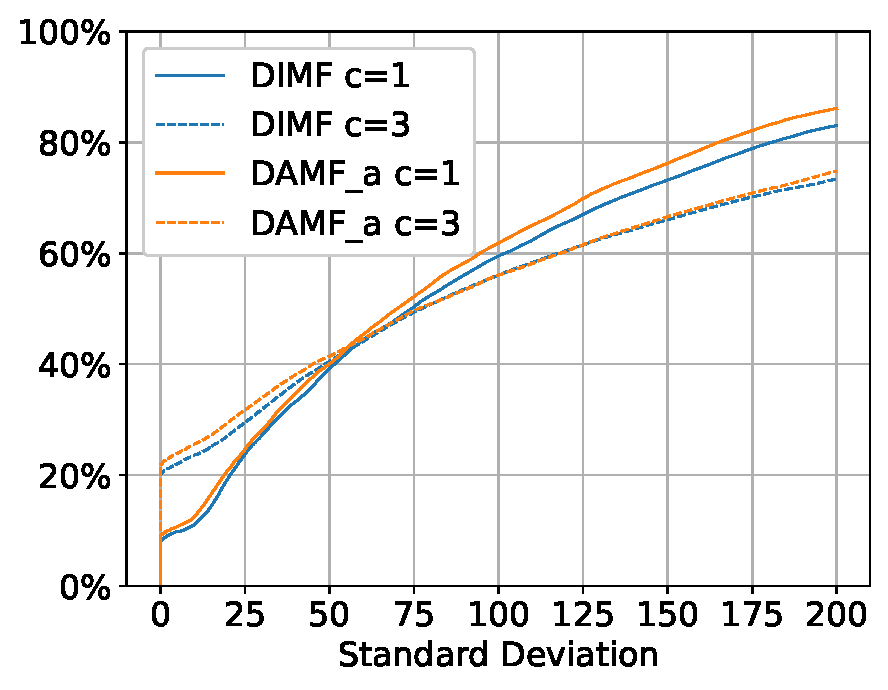
\includegraphics[width=\linewidth]{Image/SD_Ali2017test_Alpha=1.0_40_sites=50.eps}
  \caption{$m=50$}
  \label{Fg:SD_Ali_40_50m}
\end{subfigure}
\hfill
% 子图 3
\begin{subfigure}[b]{0.31\linewidth}
  \centering
  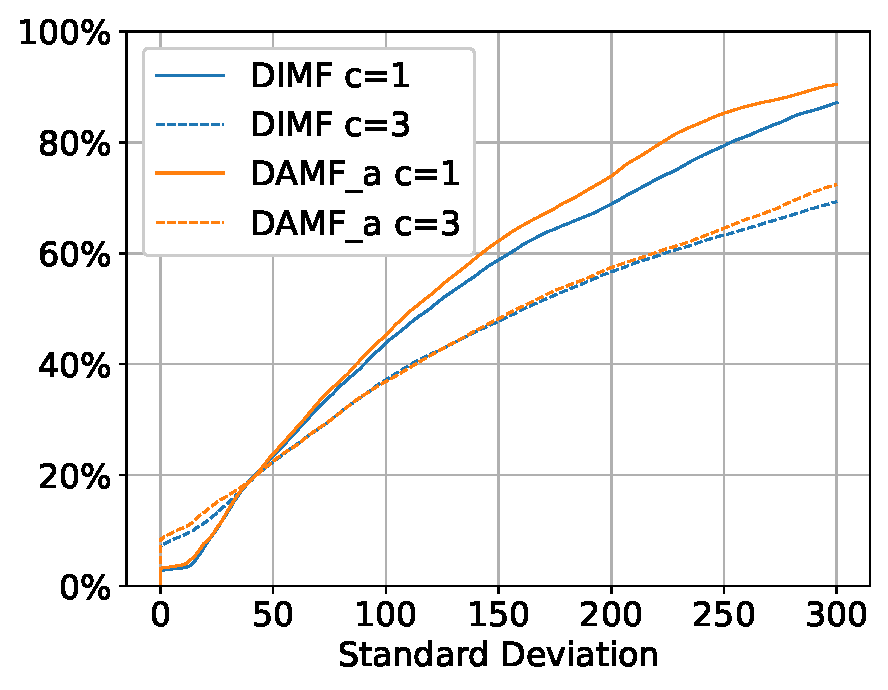
\includegraphics[width=\linewidth]{Image/SD_Ali2017test_Alpha=1.0_40_sites=100.eps}
  \caption{$m=100$}
  \label{Fg:SD_Ali_40_100m}
\end{subfigure}
\caption{Cumulative distribution of standard deviation, Alibaba, workload = 40\%, Zipf parameter $\alpha = 1$}
\label{fig:SD_sites1}
\end{figure*}

\begin{figure*}[t]
\centering
% 子图 1
\begin{subfigure}[b]{0.31\linewidth}
  \centering
  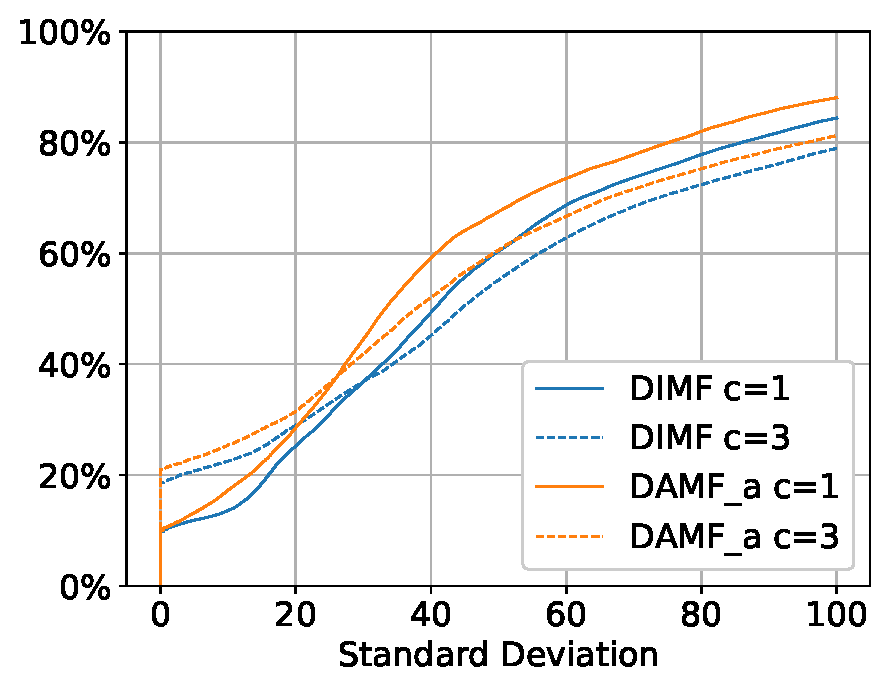
\includegraphics[width=\linewidth]{Image/SD_Ali2017test_Alpha=1.0_60_sites=20.eps}
  \caption{$m=20$}
  \label{Fg:SD_Ali_60_20m}
\end{subfigure}
\hfill % 用 \hfill 代替 \hfil，自动拉开完美的间距
% 子图 2
\begin{subfigure}[b]{0.31\linewidth}
  \centering
  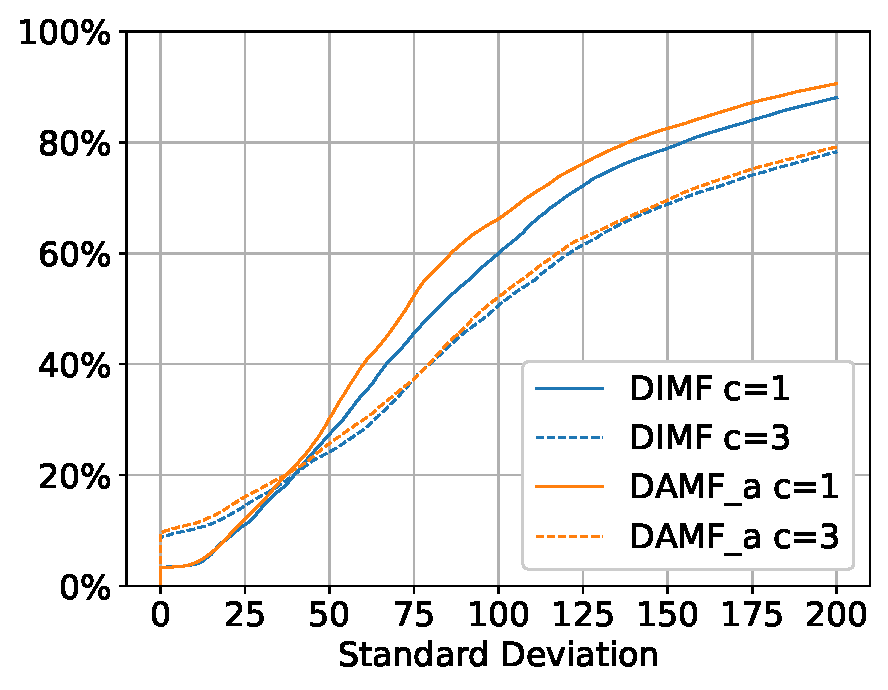
\includegraphics[width=\linewidth]{Image/SD_Ali2017test_Alpha=1.0_60_sites=50.eps}
  \caption{$m=50$}
  \label{Fg:SD_Ali_60_50m}
\end{subfigure}
\hfill
% 子图 3
\begin{subfigure}[b]{0.31\linewidth}
  \centering
  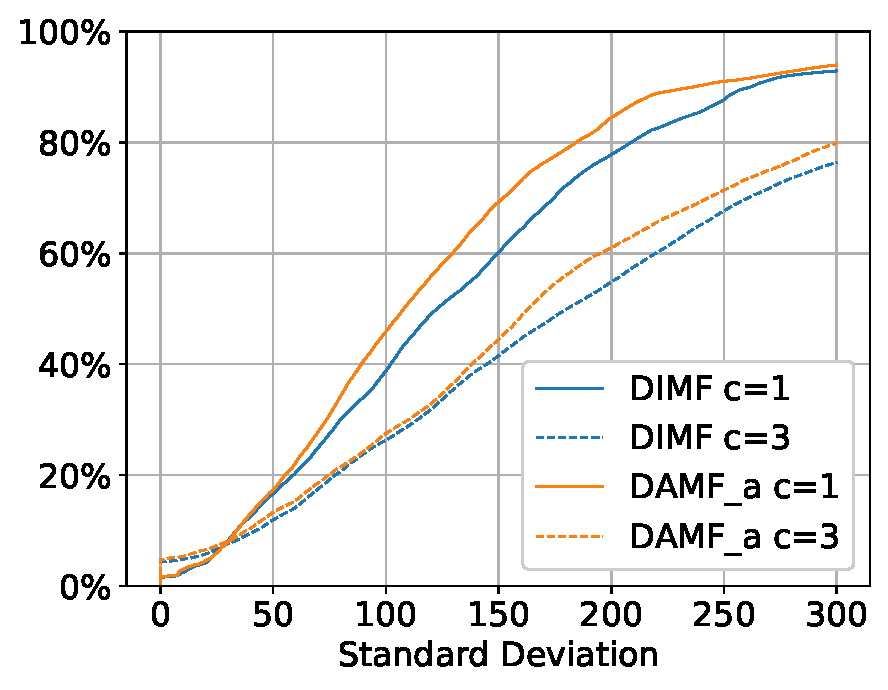
\includegraphics[width=\linewidth]{Image/SD_Ali2017test_Alpha=1.0_60_sites=100.eps}
  \caption{$m=100$}
  \label{Fg:SD_Ali_60_100m}
\end{subfigure}

\caption{Cumulative distribution of standard deviation, Alibaba, workload = 60\%, Zipf parameter $\alpha = 1$}
\label{fig:SD_sites2}
\end{figure*}

% \begin{figure}[t]
%   \centering
%   \begin{minipage}[b]{0.48\textwidth}
%     \centering
%     \subfloat[Alibaba, workload = 40\%]
%     {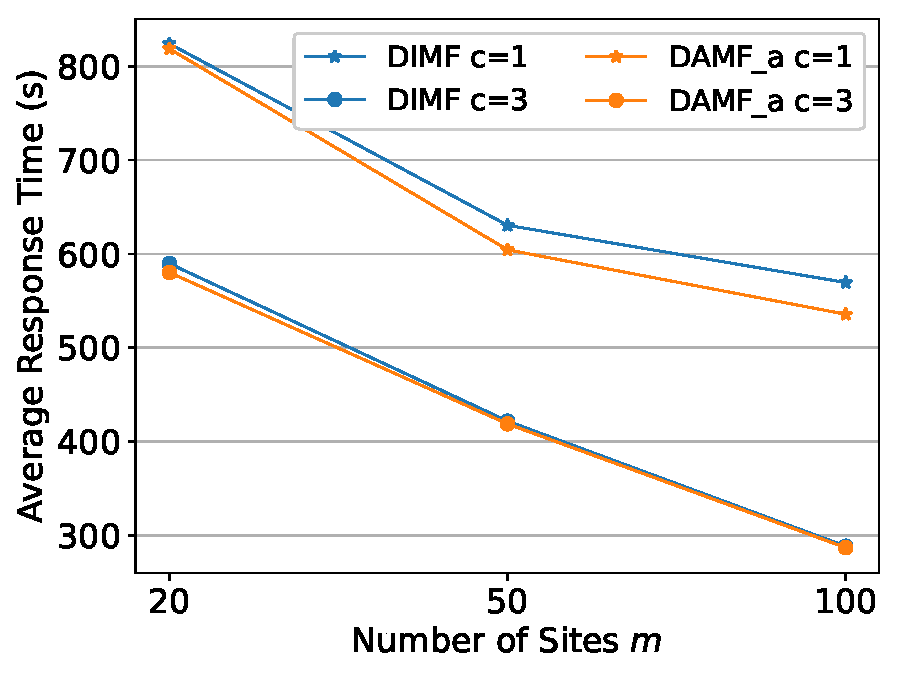
\includegraphics[width=0.48\linewidth]{Image/Workload_Ali2017test_40_site.eps}%
%     \label{Fg:JRT_Ali_40_m}
%     }
%     \hfil
%     \subfloat[Alibaba, workload = 60\%]
%     {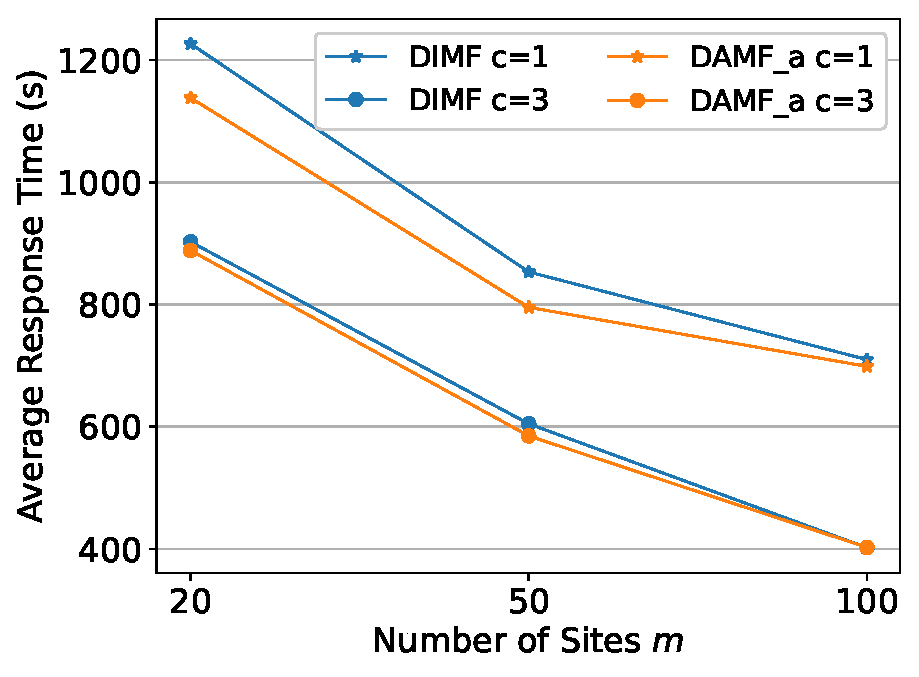
\includegraphics[width=0.48\linewidth]{Image/Workload_Ali2017test_60_site.eps}%
%     \label{Fg:JRT_Ali_60_m}
%     }
%     \caption{Average job response time, Zipf parameter $\alpha=1$}
%     \label{fig:Average Response Time_sites}
%   \end{minipage}
%   \hfill 
%   \begin{minipage}[b]{0.48\textwidth}
%     \centering
%     \subfloat[Alibaba, workload = 40\%]
%     {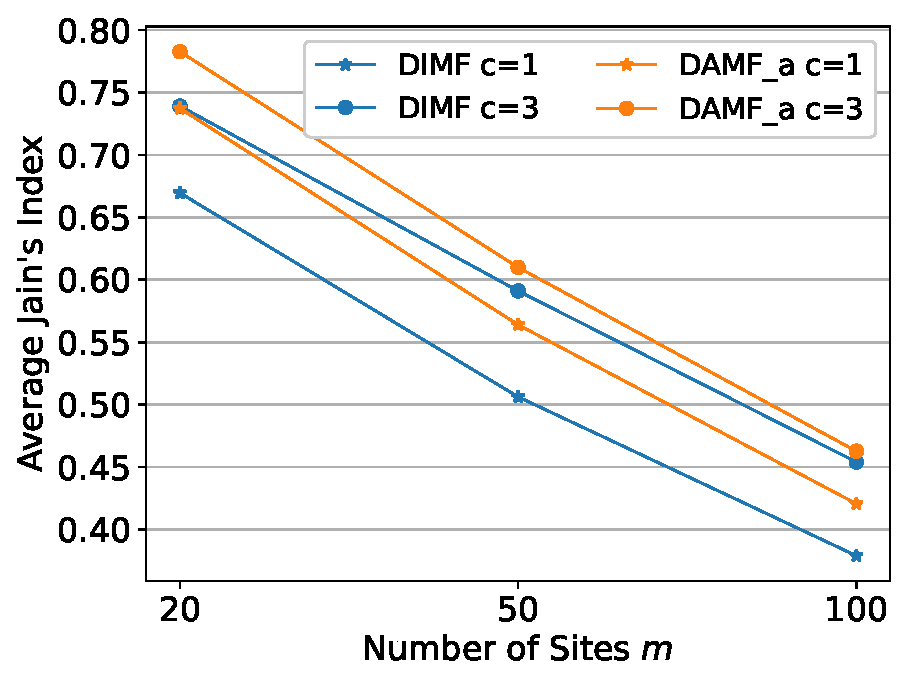
\includegraphics[width=0.48\linewidth]{Image/Jains_Ali2017test_40_site.eps}%
%     \label{Fg:Jains_Ali_40_m} % 
%     }
%     \hfil
%     \subfloat[Alibaba, workload = 60\%]
%     {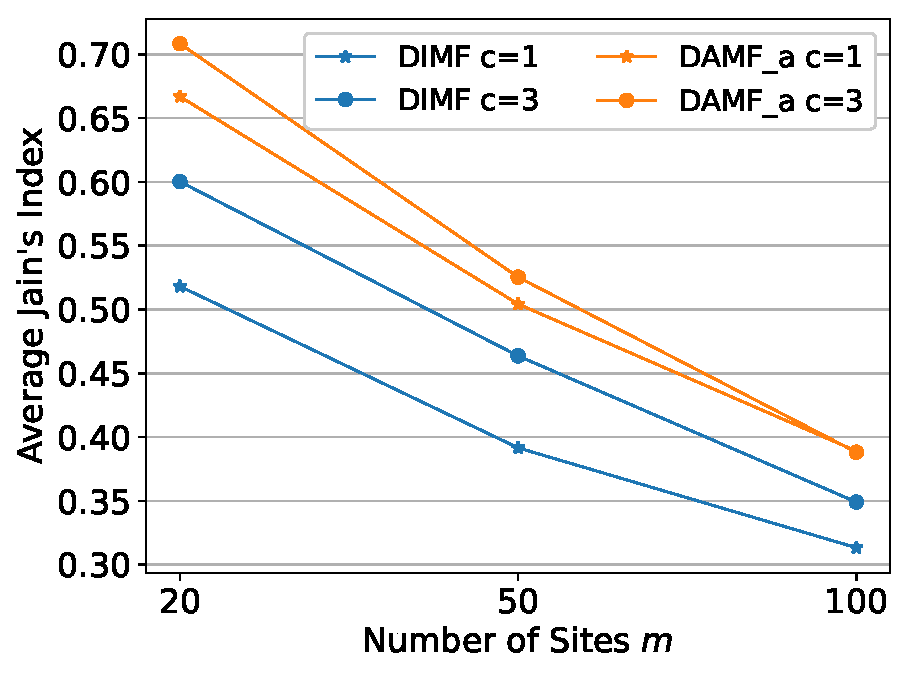
\includegraphics[width=0.48\linewidth]{Image/Jains_Ali2017test_60_site.eps}%
%     \label{Fg:Jains_Ali_60_m} % 
%     }
%     \caption{Average Jain's Index, Zipf parameter $\alpha=1$}
%     \label{fig:Jains_sites}
%   \end{minipage}
% \end{figure}

\begin{figure}[t]
    \centering
    \subfloat[Alibaba, workload = 40\%]
    {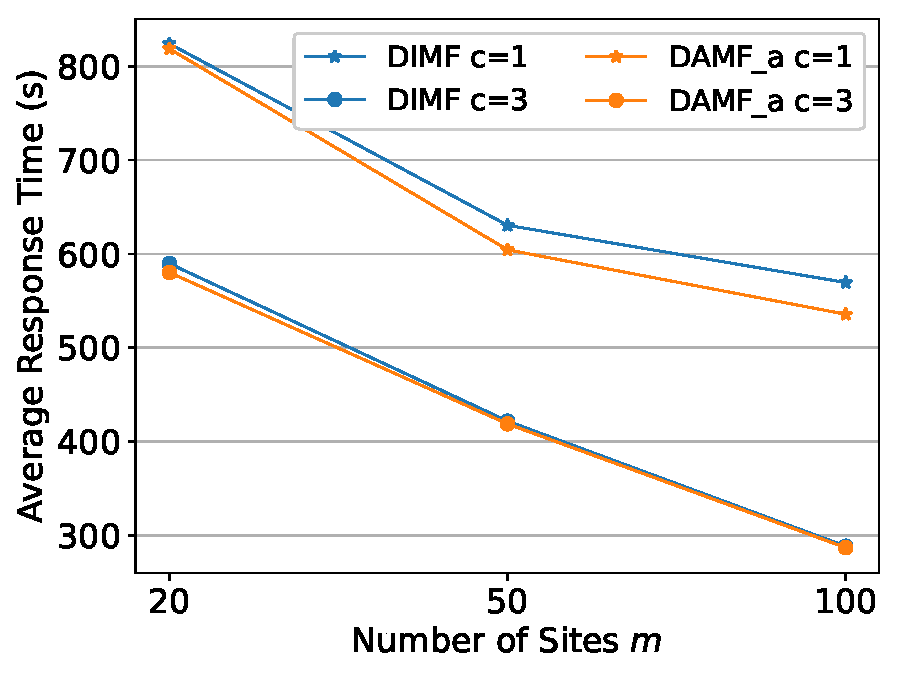
\includegraphics[width=0.48\linewidth]{Image/Workload_Ali2017test_40_site.eps}
    \label{Fg:JRT_Ali_40_m}}
    \hfill
    \subfloat[Alibaba, workload = 60\%]
    {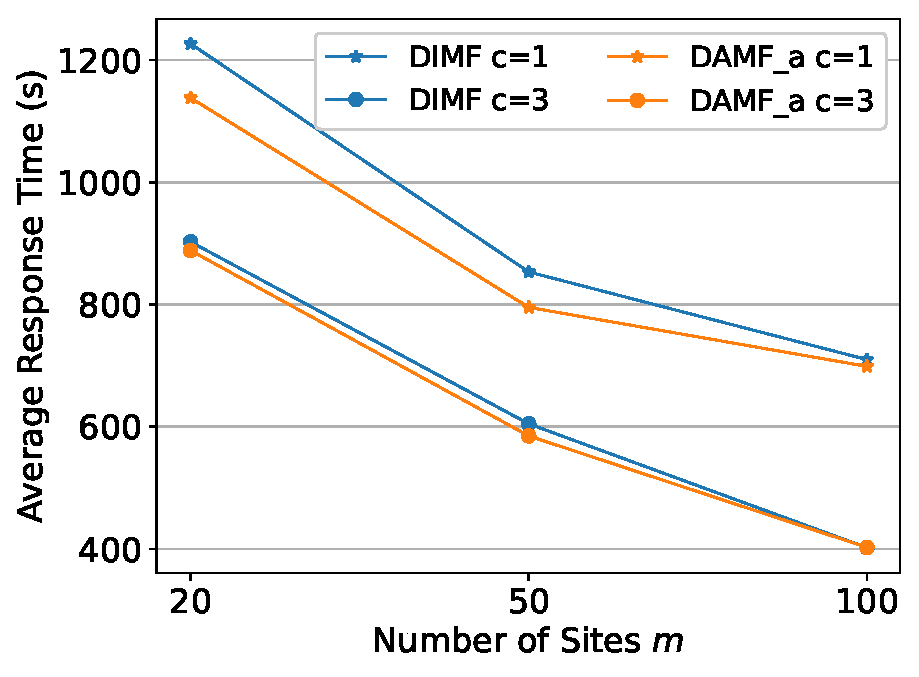
\includegraphics[width=0.48\linewidth]{Image/Workload_Ali2017test_60_site.eps}
    \label{Fg:JRT_Ali_60_m}}

    \caption{Average job response time, Zipf parameter $\alpha=1$.}
    \label{fig:Average_Response_Time_sites}
\end{figure}

\begin{figure}[t]
    \centering
    \subfloat[Alibaba, workload = 40\%]
    {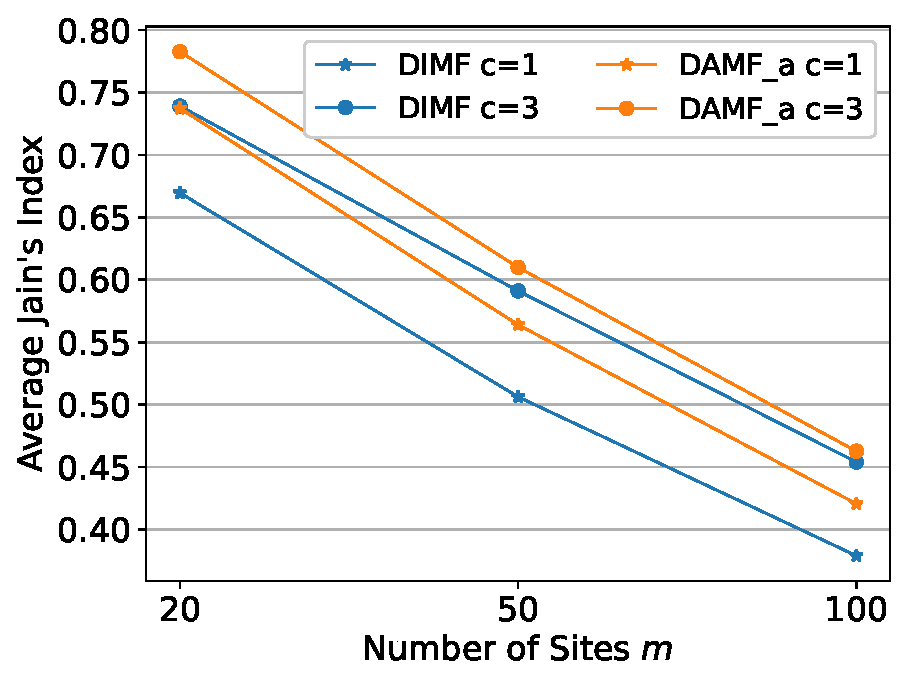
\includegraphics[width=0.48\linewidth]{Image/Jains_Ali2017test_40_site.eps}
    \label{Fg:Jains_Ali_40_m}}
    \hfill
    \subfloat[Alibaba, workload = 60\%]
    {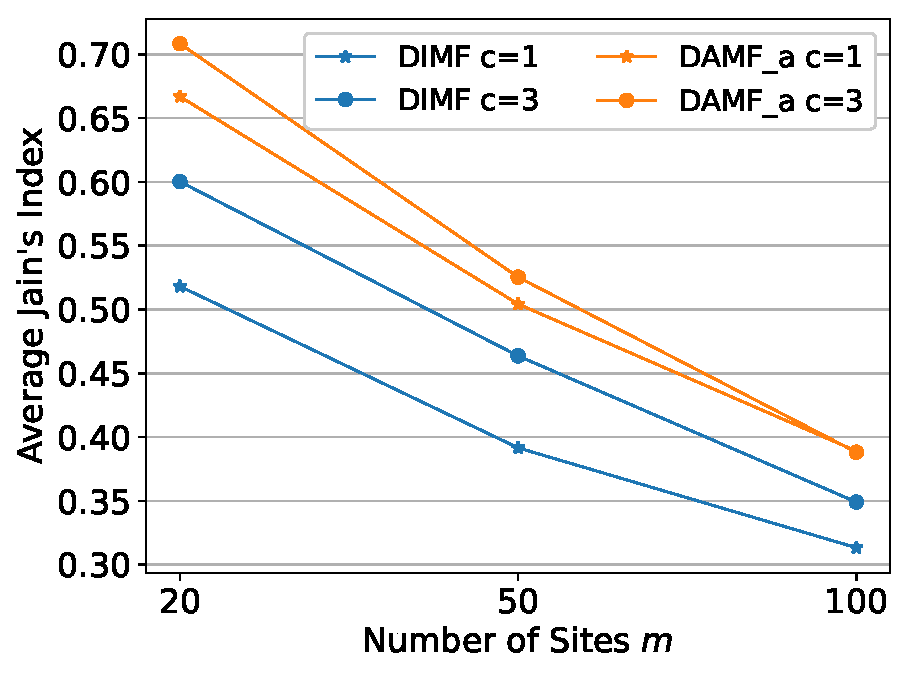
\includegraphics[width=0.48\linewidth]{Image/Jains_Ali2017test_60_site.eps}
    \label{Fg:Jains_Ali_60_m}}

    \caption{Average Jain's Index, Zipf parameter $\alpha=1$.}
    \label{fig:Jains_sites}
\end{figure}

% \begin{table}[!ht]
%   \caption{Average computation time (s) of $\text{DAMF}_a$}
%   \label{tab:computation_time_m}
%   \centering
%   \small 
%   \setlength{\tabcolsep}{4pt} 
%   \begin{tabular}{cc *{6}{S[table-format=1.3e-1]}}
%     \toprule
%     & & \multicolumn{3}{c}{Alibaba, workload = 40\%} & \multicolumn{3}{c}{Alibaba, workload = 60\%} \\
%     \cmidrule(lr){3-5} \cmidrule(lr){6-8} % 画出有间隙的分隔线，更好看
%     $c$ & $\alpha$ & {$m=20$} & {$m=50$} & {$m=100$} & {$m=20$} & {$m=50$} & {$m=100$} \\
%     \midrule
%     \multirow{4}{*}{1} 
%     & 0.0 & 2.035e-5 & 4.908e-5 & 8.455e-5 & 3.732e-5 & 7.321e-5 & 1.594e-4 \\
%     & 0.5 & 2.231e-5 & 4.491e-5 & 7.954e-5 & 3.339e-5 & 6.835e-5 & 1.592e-4 \\
%     & 1.0 & 1.645e-5 & 4.084e-5 & 7.899e-5 & 2.517e-5 & 6.675e-5 & 1.439e-4 \\
%     & 2.0 & 1.586e-5 & 3.561e-5 & 8.723e-5 & 2.243e-5 & 5.335e-5 & 1.219e-4 \\
%     \midrule
%     \multirow{4}{*}{3} 
%     & 0.0 & 2.169e-5 & 4.678e-5 & 9.114e-5 & 3.644e-5 & 7.452e-5 & 1.639e-4 \\
%     & 0.5 & 2.195e-5 & 5.027e-5 & 1.062e-4 & 3.089e-5 & 7.945e-5 & 2.174e-4 \\
%     & 1.0 & 1.836e-5 & 5.408e-5 & 1.137e-4 & 3.035e-5 & 9.177e-5 & 2.428e-4 \\
%     & 2.0 & 1.935e-5 & 5.155e-5 & 1.443e-4 & 2.786e-5 & 9.714e-5 & 2.868e-4 \\
%     \bottomrule
%   \end{tabular}
% \end{table}

\begin{table}[!ht]
  \caption{Average computation time (s) of $\text{DAMF}\_a$}
  \label{tab:computation_time_m}
  \centering
  \resizebox{\columnwidth}{!}{
  \setlength{\tabcolsep}{4pt} 
  \begin{tabular}{cc *{6}{S[table-format=1.3e-2, input-exponent-markers={e}]}}
    \toprule
    & & \multicolumn{3}{c}{Alibaba, workload = 40\%} & \multicolumn{3}{c}{Alibaba, workload = 60\%} \\
    \cmidrule(lr){3-5} \cmidrule(lr){6-8} 
    $c$ & $\alpha$ & {$m=20$} & {$m=50$} & {$m=100$} & {$m=20$} & {$m=50$} & {$m=100$} \\
    \midrule
    \multirow{4}{*}{1} 
    & 0.0 & 2.035e-5 & 4.908e-5 & 8.455e-5 & 3.732e-5 & 7.321e-5 & 1.594e-4 \\
    & 0.5 & 2.231e-5 & 4.491e-5 & 7.954e-5 & 3.339e-5 & 6.835e-5 & 1.592e-4 \\
    & 1.0 & 1.645e-5 & 4.084e-5 & 7.899e-5 & 2.517e-5 & 6.675e-5 & 1.439e-4 \\
    & 2.0 & 1.586e-5 & 3.561e-5 & 8.723e-5 & 2.243e-5 & 5.335e-5 & 1.219e-4 \\
    \midrule
    \multirow{4}{*}{3} 
    & 0.0 & 2.169e-5 & 4.678e-5 & 9.114e-5 & 3.644e-5 & 7.452e-5 & 1.639e-4 \\
    & 0.5 & 2.195e-5 & 5.027e-5 & 1.062e-4 & 3.089e-5 & 7.945e-5 & 2.174e-4 \\
    & 1.0 & 1.836e-5 & 5.408e-5 & 1.137e-4 & 3.035e-5 & 9.177e-5 & 2.428e-4 \\
    & 2.0 & 1.935e-5 & 5.155e-5 & 1.443e-4 & 2.786e-5 & 9.714e-5 & 2.868e-4 \\
    \bottomrule
  \end{tabular}}
\end{table}

\section{Summary}
\label{sec:ch3summary}
In this chapter, we have defined a new resource allocation policy called Dynamic Aggregate Max-min Fairness (DAMF) in distributed job execution with task transmissions. We prove that DAMF satisfies several widely accepted properties, including Pareto efficiency, envy-freeness and strategy-proofness. We present an algorithm for computing the DAMF allocation and a fast approximation. Experimental evaluations using real job traces from Alibaba and Google demonstrate that DAMF could effectively enhance the fairness of resource allocation among jobs and improve the system utility. %In the future, we plan to extend our work to deal with multiple resource types.

% \section*{Acknowledgments}
% This research is supported by the Ministry of Education, Singapore, under its Academic Research Fund Tier 2 (Award MOE-T2EP20121-0005) and Academic Research Fund Tier 1 (Award RG23/23).